\chapter{Quantum sensing networks and the role of correlations}
\label{chap:networks}

\section{Goals for the third stage of our methodology}
\label{sec:goals6}

While the methods in the two previous chapters can be applied to a wide range of single-parameter problems, in section \ref{subsec:multischemes} we argued that more realistic scenarios typically involve several pieces of unknown information; consequently, the next step is to accommodate our ideas to this type of schemes, and in this chapter we will generalise the hybrid estimation approach in chapter \ref{chap:nonasymptotic} to the multi-parameter regime. Given that the transition from single-parameter metrology to multi-parameter schemes opens the door to a vast set of new ways of enhancing our estimation protocols \cite{chiara2003, spagnolo2012, chiribella2012, humphreys2013, zhang2014, berry2015, baumgratz2016, knott2016local, gagatos2016gaussian, Szczykulska2016, jasminder2016, proctor2017networked, proctor2017networkedshort, vidrighin2014, szczykulska2017, zhang_lu2017, altenburg2017, zhuang2017, altenburg2018, hall2018, sekatski2019, qian2019, polino2018, roccia2018, jasminder2018, ge2018, eldredge2018, li2019, gatto2019}, it is important that we first identify the subset of estimation problems that we intend to investigate here. 

Let us recall our discussion in section \ref{subsec:multischemes}, where we introduced the quantum network model for distributed sensing proposed by Proctor \emph{et al.} \cite{proctor2017networked, proctor2017networkedshort}. We will focus our attention on a collection of sensors arranged such that a single parameter $\theta_i$ is encoded in the $i$-th sensor, and we will explore whether allowing for correlations between different sensors enhances the overall precision of their estimation. In the context of this configuration, Proctor \emph{et al.} \cite{proctor2017networked, proctor2017networkedshort} have shown that, assuming that the associated generators commute, such correlations are not needed to achieve the uncertainty that is optimal when the inverse of the Fisher information matrix is employed as the figure of merit \cite{proctor2017networked, proctor2017networkedshort}. Crucially, using this measure of uncertainty could be a potential caveat to the results of their framework, since we can always achieve any value for the local variances with the class of \emph{infinite-precision} states studied in section \ref{subsec:infiniteprecision}, while, at the same time, this type of probe can require a high amount of prior knowledge to work and a large number of trials to reach the Cram\'{e}r-Rao bound. Moreover, in chapter \ref{chap:limited} we have provided compelling evidence of the existence of a potential trade-off between the performances in the asymptotic and non-asymptotic regimes. Therefore, a study of the role of entanglement for the estimation of the parameters encoded in each sensor when the network operates in the non-asymptotic regime is needed, and this is one of the multi-parameter problems that both this chapter and chapter \ref{chap:multibayes} will address.

On the other hand, if we consider that the parameters in each sensor are local properties of the network, then a collection of functions of the parameters encoded in different sensors represents global properties. In that case, entangled strategies can provide a notable advantage with respect to local schemes \cite{proctor2017networked, proctor2017networkedshort} and, as a consequence, we can say that whether local or global strategies are preferable crucially depends on the type of information that we wish to extract\footnote{A related conclusion was reached by Altenburg and W\"{o}lk in \cite{altenburg2018}, where the authors further studied sequential strategies, that is, strategies that use entangled states to estimate one global property at a time, and concluded that no type of strategy  local, global or sequential - could be claimed to be optimal in general.}. The estimation of global properties or functions is particularly relevant in problems such as the interpolation of non-linear functions \cite{qian2019} and the determination of the coefficients in Taylor or Fourier expansions of some field \cite{sekatski2019}, and, from a fundamental perspective, it is important to understand the connection between the form of the functions to be estimated and the form of the quantum strategy that yields an optimal precision. For instance, using the model for quantum sensing networks under consideration it has been established that one can find entangled states that beat the best separable probe for the optimal estimation of a single function $f(\boldsymbol{\theta})$ that is linear \cite{proctor2017networked, proctor2017networkedshort, eldredge2018, altenburg2018, qian2019, gatto2019}, while a collection of linear functions that generate an orthogonal transformation (that is, $\boldsymbol{f}(\boldsymbol{\theta}) = V^{\transpose} \boldsymbol{\theta}$ with $V V^{-1}=\mathbb{I}$) can be estimated optimally with a completely local strategy \cite{proctor2017networked}. 

This state of affairs motivates the second and main multi-parameter problem that we wish to study in this chapter. More concretely, the problem of estimating several functions will be formulated using the asymptotic theory first, and then we will take those solutions as a guide to perform a Bayesian analysis of the non-asymptotic regime for some of these schemes. While a general answer is beyond the scope of our methods, we will see that it is possible to arrive to definite conclusions by focusing on a subclass of schemes with sensor-symmetric states, and by modelling its global properties with linear but otherwise general functions. Given that configuration, we will establish and exploit the link between the geometry of the linear functions and the strength of the inter-sensor correlations of the network, and we will explore how this may change as the number of repetitions varies.

Importantly, unlike with the schemes of chapter \ref{chap:nonasymptotic}, whose asymptotically optimal quantum strategies where available in the literature, here we will solve the asymptotic estimation problem explicitly before we perform its associated Bayesian analysis. In particular, suppose we denote the number of functions by $l$, and recall that $d$ is the number of unknown parameters. If the functions can be written in terms of an orthogonal transformation, then we have that $l = d$. Hence, from the previous discussion we see that the next natural step is to search for and examine the connection between global properties and the optimal strategy for their estimation when $l\neq 1$ and $l\neq d$, or when $l = d$ and the functions are linear but not orthogonal. This new intermediate regime is precisely the case that we will consider\footnote{Note that the estimation of several functions that are not orthogonal to each other has already arisen in specific applications. An example of this can be found in \cite{li2019}, where the authors studied a protocol for Ramsey interferometry. The importance of the results in the first half of this chapter rests on the partial generality and the fundamental focus of our approach, which is based on the framework provided by the quantum sensing network model in \cite{proctor2017networked}.}.  

In summary, the third stage of our methodology, which rests on combining the multi-parameter estimator that is exactly optimal with the asymptotically optimal quantum strategy, will serve as a basis to investigate how to harness correlations in multi-parameter problems when different amounts of data are available. Note that, as in chapter \ref{chap:nonasymptotic}, our approach not only provides a characterisation of our schemes in the non-asymptotic regime, but also estimates the number of repetitions and prior knowledge needed to recover the predictions of the Cram\'{e}r-Rao bound. Since the construction and maintenance of entangled networks are likely to be difficult in practice, our proposal may prove to be crucial in the study and implementation of sensing networks that operate with a realistic amount of data. 
 
\section{Methodology (part C)}

\subsection{Relevant information in multi-parameter schemes}
\label{subsec:relevantinfo}

Let us formulate the problem of estimating several functions in terms of the information content that we wish to extract using the network\footnote{We recall that this perspective was also exploited in chapter \ref{chap:methodology} to justify the suitability of different measures of uncertainty.}.

We will assign the terminology \emph{natural or primary properties} to those parameters that appear in the physical characterisation of the scheme. These have been denoted by $\boldsymbol{\theta}$ in the first part of this work. In addition, any collection of functions of them, which we can generally denote by $\boldsymbol{f}(\boldsymbol{\theta}) = (f_1(\boldsymbol{\theta}), \dots, f_l(\boldsymbol{\theta}))$, can be seen as  a set of \emph{derived or secondary properties} that we might wish to find. Importantly, there is a degree of arbitrariness in deciding which quantities are primary and which ones are secondary, and this should be fixed by the concrete application under analysis. For example, in previous chapters we have considered that the difference of optical phase shifts in a Mach-Zehnder interferometer is the natural parameter, instead of considering each phase shift independently and the difference as a function of them. 

The information that characterises the network is complete once we know all the natural parameters. In that case, we could also calculate any function of them. However, if the functions of interest only depend on some parameters, or they only require a particular combination of the primary properties, then it is not necessary nor optimal to spend resources in gathering all the information about the original parameters \cite{proctor2017networked}, since only certain pieces of information are relevant to us. In other words, studying functions of the original parameters is effectively equivalent to selecting which information the network should be focused on, so that we can optimise it accordingly.  For that reason, the specific form of the functions, i.e., $\boldsymbol{f}(\cdot)$, will be assumed to be known. 

In turn, this motivates the use of $\boldsymbol{f}[\boldsymbol{g}(\boldsymbol{m})] = (f_1[\boldsymbol{g}(\boldsymbol{m})], \dots, f_l[\boldsymbol{g}(\boldsymbol{m})])$ as the vector estimator for the functions, where we recall that $\boldsymbol{g}(\boldsymbol{m})$ are the estimators for the natural parameters. Although in principle we could consider more general estimators for the derived properties \cite{gill2011}, this choice is appropriate to highlight that the functions are part of the specification of the problem, and that the information is partial only due to the lack of knowledge about the parameters. Then, given some reasonable deviation function $\mathcal{D}\left[\boldsymbol{g}(\boldsymbol{m}), \boldsymbol{\theta}, \boldsymbol{f}(\cdot), \mathcal{W}_f \right]$ for the estimation of derived or secondary properties, we can approximate it with the square error as
\begin{eqnarray}
\mathcal{D}\left[\boldsymbol{g}(\boldsymbol{m}), \boldsymbol{\theta}, \boldsymbol{f}(\cdot), \mathcal{W}_f \right] \approx \mathrm{Tr}\left( \mathcal{W}_f \left\lbrace\boldsymbol{f}[\boldsymbol{g}(\boldsymbol{m})] - \boldsymbol{f}(\boldsymbol{\theta}) \right\rbrace \left\lbrace\boldsymbol{f}[\boldsymbol{g}(\boldsymbol{m})] - \boldsymbol{f}(\boldsymbol{\theta}) \right\rbrace^\transpose \right),
\label{errfunctions}
\end{eqnarray}
for a moderate amount of prior knowledge about the primary properties, where the weighting matrix for the functions is $\mathcal{W}_f = \mathrm{diag}(w_1, \cdots, w_l)$. Note that if the nature of the functions is such that the square error generates an appropriate measure of uncertainty, then the approximation in equation (\ref{errfunctions}) becomes an equality.  

To make the problem more tractable, we will assume that the secondary properties are linear, that is, $\boldsymbol{f}(\boldsymbol{\theta}) = V^{\transpose} \boldsymbol{\theta} + \boldsymbol{a}$, where $V$ is a $(d\times l)$ matrix and $\boldsymbol{a}$ is a column vector with $l$ components. In that case, the error in equation (\ref{errfunctions}) becomes
\begin{equation}
\mathcal{D}\left[\boldsymbol{g}(\boldsymbol{m}), \boldsymbol{\theta}, \boldsymbol{f}(\cdot), \mathcal{W}_f \right] \approx \mathrm{Tr}\left\lbrace \mathcal{W}_f  V^{\transpose} \left[\boldsymbol{g}(\boldsymbol{m}) - \boldsymbol{\theta}\right] \left[\boldsymbol{g}(\boldsymbol{m}) - \boldsymbol{\theta}\right]^\transpose  V \right\rbrace.
\label{errlinfun}
\end{equation}
The fact that it does not depend on $\boldsymbol{a}$ allows us to set $\boldsymbol{a} = \boldsymbol{0}$ without loss of generality. Thus the functions are simply $\boldsymbol{f}(\boldsymbol{\theta}) = V^{\transpose}\boldsymbol{\theta}$, such that the coefficients are encoded in the columns of $V$. 

The previous formalism is reduced to some of the extreme cases that have been studied by other authors (e.g., in \cite{proctor2017networked, proctor2017networkedshort, altenburg2018}). In particular, equation (\ref{errlinfun}) includes the estimation of a single function when $V$ is chosen as a column vector, and a collection of $l = d$ orthogonal functions is equivalent to imposing that $V$ is an orthogonal matrix. Note that, in the latter case, $\mathcal{W}_f = \mathrm{diag}(w_1, \dots, w_d) = \mathcal{W}$. Moreover, if the orthogonal transformation happens to be the identity, i.e., $V = \mathbb{I}$, then we recover the deviation function for the natural parameters in equation (\ref{multideviation}). However, this framework also covers a rich spectrum of possibilities where any number of linear but otherwise general functions are allowed. Therefore, it is clear that, despite our linearity assumption, this approach will allow us to explore the new regime described in section \ref{sec:goals6}.

Once we have selected a suitable deviation function for the multi-parameter problem of estimating functions, we can finally construct the measure of uncertainty 
\begin{eqnarray}
\bar{\epsilon}_{\mathrm{mse}} = \int d\boldsymbol{\theta} d\boldsymbol{m} ~p(\boldsymbol{\theta}, \boldsymbol{m})~\mathrm{Tr}\left\lbrace \mathcal{W}_f V^\transpose \left[\boldsymbol{g}(\boldsymbol{m}) - \boldsymbol{\theta}\right] \left[\boldsymbol{g}(\boldsymbol{m}) - \boldsymbol{\theta}\right]^\transpose V \right\rbrace
\label{msefunctions}
\end{eqnarray}
that is to be optimised. 

\subsection{The asymptotic regime for many parameters}
\label{subsec:multiasymp}

We start by optimising equation (\ref{msefunctions}) over all the possible vector estimators. First we rewrite it as 
\begin{align}
\bar{\epsilon}_\mathrm{mse} &= \mathrm{Tr}\left(\mathcal{W}_f V^\transpose \Sigma_\mathrm{mse} V\right) = \sum_{i=1}^l \sum_{j=1}^d \left(\mathcal{W}_f V^\transpose \Sigma_\mathrm{mse}\right)_{ij}V_{ji}
\nonumber \\
&= \sum_{j=1}^d \sum_{i=1}^l V_{ji} \left(\mathcal{W}_f V^\transpose \Sigma_\mathrm{mse}\right)_{ij} = \mathrm{Tr}\left(V \mathcal{W}_f V^\transpose \Sigma_\mathrm{mse}\right),
\end{align}
where we have defined the matrix square error
\begin{equation}
\Sigma_\mathrm{mse} = \int d\boldsymbol{\theta} d\boldsymbol{m} ~p(\boldsymbol{\theta}, \boldsymbol{m}) \left[\boldsymbol{g}(\boldsymbol{m}) - \boldsymbol{\theta}\right] \left[\boldsymbol{g}(\boldsymbol{m}) - \boldsymbol{\theta}\right]^\transpose.
\label{matrixmse}
\end{equation}
Given that both $V \mathcal{W}_f V^\transpose$ and $\Sigma_\mathrm{mse}$ are symmetric positive semi-definite matrices\footnote{That $V \mathcal{W}_f V^\transpose$ is symmetric can be easily verified as
\begin{align}
\left(V \mathcal{W}_f V^\transpose \right)^\transpose &= \left(\sum_{i,m=1}^d \sum_{k,j=1}^l V_{ij} (\mathcal{W}_f)_{jk} V_{mk} \boldsymbol{e}_i \boldsymbol{e}_m^\transpose\right)^\transpose = \sum_{i,m=1}^d \sum_{k,j=1}^l V_{ik} (\mathcal{W}_f)_{jk} V_{mj} \boldsymbol{e}_i \boldsymbol{e}_m^\transpose 
\nonumber \\
&= V \mathcal{W}_f^\transpose V^\transpose = V \mathcal{W}_f V^\transpose,
\nonumber
\end{align}
where $\boldsymbol{e}_i$ is the $i$-th element of the basis, while its positive semi-definiteness arises from the fact that, for any $\boldsymbol{u}$,
\begin{align}
\boldsymbol{u}^\transpose V \mathcal{W}_f V^\transpose \boldsymbol{u} &= \sum_{i, m = 1}^d \sum_{j, k = 1}^l u_i V_{ij} (\mathcal{W}_f)_{jk} V_{mk} u_m = \sum_{i, m = 1}^d \sum_{j = 1}^l u_i V_{ij} w_j V_{mj} u_m 
\nonumber \\
&= \sum_{j = 1}^l w_j \left(\sum_{i=1}^d u_i V_{ij} \right)^2 \geqslant 0.
\nonumber
\end{align}}, we can find the minimum value for $\bar{\epsilon}_\mathrm{mse}$ simply by searching for the estimators that make $\Sigma_{\mathrm{mse}}$ minimal in the matrix sense. In other words, we need to show that $\boldsymbol{u}^\transpose \Sigma_{\mathrm{mse}} \boldsymbol{u} \geqslant \boldsymbol{u}^\transpose C \boldsymbol{u}$ for an arbitrary real vector $\boldsymbol{u}$ and some symmetric positive semi-definite matrix $C$ that arises after selecting the optimal estimators\footnote{To see why this method works, note that, if $(\Sigma_{\mathrm{mse}} - C) \geqslant 0$, then
\begin{align}
\mathrm{Tr}\left[V \mathcal{W}_f V^\transpose \left(\Sigma_{\mathrm{mse}} - C \right)\right] &= \mathrm{Tr}\left(\sqrt{V \mathcal{W}_f V^\transpose}\sqrt{V \mathcal{W}_f V^\transpose} \sqrt{\Sigma_{\mathrm{mse}} - C }\sqrt{\Sigma_{\mathrm{mse}} - C }\right)
\nonumber \\
&= \mathrm{Tr}\left(\sqrt{V \mathcal{W}_f V^\transpose} \sqrt{\Sigma_{\mathrm{mse}} - C }\sqrt{\Sigma_{\mathrm{mse}} - C }\sqrt{V \mathcal{W}_f V^\transpose} \right)
\nonumber \\
&= \mathrm{Tr}\left[\sqrt{V \mathcal{W}_f V^\transpose} \sqrt{\Sigma_{\mathrm{mse}} - C }\left(\sqrt{V \mathcal{W}_f V^\transpose} \sqrt{\Sigma_{\mathrm{mse}} - C }\right)^\transpose \right]
\nonumber \\
&= \sum_{i,j = 1}^d \left(\sqrt{V \mathcal{W}_f V^\transpose} \sqrt{\Sigma_{\mathrm{mse}} - C }\right)_{ij}^2 \geqslant 0,
\nonumber
\end{align}
which implies that 
\begin{equation}
\bar{\epsilon}_{\mathrm{mse}} = \mathrm{Tr}\left(V \mathcal{W}_f V^\transpose \Sigma_{\mathrm{mse}}\right) \geqslant \mathrm{Tr}\left(V \mathcal{W}_f V^\transpose C\right).
\nonumber
\end{equation}
}.

Our task is then to minimise the scalar quantity
\begin{equation}
\boldsymbol{u}^\transpose \Sigma_{\mathrm{mse}} \boldsymbol{u} = \int d\boldsymbol{\theta} d\boldsymbol{m} ~p(\boldsymbol{\theta}, \boldsymbol{m}) \left[g_u(\boldsymbol{m}) - \theta_u  \right]^2,
\label{scalarquantitynetworks}
\end{equation}
with $g_u(\boldsymbol{m}) = \boldsymbol{u}^\transpose \boldsymbol{g}(\boldsymbol{m}) = \boldsymbol{g}^\transpose(\boldsymbol{m})  \boldsymbol{u}$, $\theta_u = \boldsymbol{u}^\transpose \boldsymbol{\theta} = \boldsymbol{\theta}^\transpose \boldsymbol{u}$ and arbitrary $\boldsymbol{u}$. Since $\boldsymbol{u}^\transpose \Sigma_{\mathrm{mse}} \boldsymbol{u}$ is a functional of $g_u(\boldsymbol{m})$, we can formulate another variational problem as
\begin{equation}
\delta \epsilon\left[g_u(\boldsymbol{m})\right] = \delta \int d\boldsymbol{m}~\mathcal{L}\left[\boldsymbol{m}, g_u(\boldsymbol{m}) \right] = 0,
\end{equation} 
where $\epsilon\left[g_u(\boldsymbol{m})\right] = \boldsymbol{u}^\transpose \Sigma_{\mathrm{mse}} \boldsymbol{u}$ and $\mathcal{L}\left[m, g_u(\boldsymbol{m}) \right] = \int d\boldsymbol{\theta} p(\boldsymbol{\theta}, \boldsymbol{m}) \left[g_u(\boldsymbol{m}) - \theta_u  \right]^2 $. Formally, this is the same type of calculation found in sections \ref{subsec:originalderivation} and \ref{theory}. As such, we know that the solution that makes $ \epsilon\left[g_u(\boldsymbol{m})\right]$ extremal is $g_u(\boldsymbol{m}) = \int d\boldsymbol{\theta} p(\boldsymbol{\theta}|\boldsymbol{m})\theta_u$, with $p(\boldsymbol{\theta}|\boldsymbol{m}) \propto p(\boldsymbol{\theta})p(\boldsymbol{m}|\boldsymbol{\theta})$, and we can expand it as 
\begin{equation}
\sum_{i=1}^d u_i \left[g_i\left(\boldsymbol{m}\boldsymbol\right) - \int d\boldsymbol{\theta} p(\boldsymbol{\theta}|\boldsymbol{m}) \theta_i \right] = 0.
\label{optmultiestimator}
\end{equation}
We also know that equation (\ref{optmultiestimator}) gives rise to a minimum; consequently, by inserting this solution in equation (\ref{scalarquantitynetworks}) we find that $\boldsymbol{u}^\transpose \Sigma_{\mathrm{mse}} \boldsymbol{u}$ is lower bounded by
\begin{equation}
\boldsymbol{u}^\transpose \int d\boldsymbol{m}~ p(\boldsymbol{m}) \left\lbrace \int d\boldsymbol{\theta} p(\boldsymbol{\theta}|\boldsymbol{m}) \boldsymbol{\theta}\boldsymbol{\theta}^\transpose - \left[\int d\boldsymbol{\theta} p(\boldsymbol{\theta}|\boldsymbol{m}) \boldsymbol{\theta}\right] \left[\int d\boldsymbol{\theta} p(\boldsymbol{\theta}|\boldsymbol{m}) \boldsymbol{\theta}\right]^\transpose \right\rbrace \boldsymbol{u},
\label{multiclassicalcondition}
\end{equation}
where $p(\boldsymbol{m}) = \int d\boldsymbol{\theta} p(\boldsymbol{\theta})p(\boldsymbol{m}|\boldsymbol{\theta})$. 

Equation (\ref{multiclassicalcondition}) must be less than or equal to $\boldsymbol{u}^\transpose \Sigma_{\mathrm{mse}} \boldsymbol{u}$ for any $\boldsymbol{u}$. As such, we conclude that the minimum matrix error is
\begin{equation}
\Sigma_\mathrm{mse} =  \int d\boldsymbol{m}~ p(\boldsymbol{m}) \Sigma(\boldsymbol{m}),
\label{matrixmsemin}
\end{equation}
with 
\begin{equation}
\Sigma(\boldsymbol{m}) = \int d\boldsymbol{\theta} p(\boldsymbol{\theta}|\boldsymbol{m}) \boldsymbol{\theta}\boldsymbol{\theta}^\transpose - \left[\int d\boldsymbol{\theta} p(\boldsymbol{\theta}|\boldsymbol{m}) \boldsymbol{\theta}\right] \left[\int d\boldsymbol{\theta} p(\boldsymbol{\theta}|\boldsymbol{m}) \boldsymbol{\theta}\right]^\transpose,
\end{equation}
and that this is achieved for the optimal vector estimator $\boldsymbol{g}\left(\boldsymbol{m}\right) = \int d\boldsymbol{\theta} p(\boldsymbol{\theta}|\boldsymbol{m}) \boldsymbol{\theta}$, in agreement with what is known in the literature \cite{kay1993}. Furthermore, combining equation (\ref{matrixmsemin}) with the original uncertainty in equation (\ref{msefunctions}), and expanding the result of that operation in components, we find that the minimum error for the estimation of the functions is 
\begin{eqnarray}
\bar{\epsilon}_{\mathrm{mse}} = \sum_{i=1}^l w_i \int d\boldsymbol{m}~ p(\boldsymbol{m}) \left\lbrace \int d\boldsymbol{\theta} p(\boldsymbol{\theta}|\boldsymbol{m}) f_i^2(\boldsymbol{\theta}) - \left[\int d\boldsymbol{\theta} p(\boldsymbol{\theta}|\boldsymbol{m}) f_i(\boldsymbol{\theta})\right]^2 \right\rbrace,
\label{msefunctionsmin}
\end{eqnarray}
where $f_i(\boldsymbol{\theta}) = \sum_{j=1}^d V_{ji} \theta_j$. This is the central quantity of this chapter.

Next we wish to select the quantum strategy that is asymptotically optimal, so that we need to examine the asymptotic behaviour of equation (\ref{msefunctionsmin}). This study mimics the strategy that we employed in section \ref{theory} for the scalar case, for which we followed the works \cite{jaynes2003, cox2000, bernardo1994}, and we also do it here. 

Suppose there is a region of the multi-parameter domain with hypervolume $\Delta$ where the likelihood $p(\boldsymbol{m}|\boldsymbol{\theta})$ becomes concentrated around an absolute maximum $\boldsymbol{\theta}_{\boldsymbol{m}}$ as $\mu \rightarrow \infty$, and that the prior for the primary properties is approximately flat in such region. Furthermore, the true vector parameter is $\boldsymbol{\theta}'$. In this regime we can then approximate $\mathrm{log}[p(\boldsymbol{m}|\boldsymbol{\theta})]$ formally as 
\begin{align}
\mathrm{log}[p(\boldsymbol{m}|\boldsymbol{\theta})] \approx  &~\mathrm{log}[p(\boldsymbol{m}|\boldsymbol{\theta}_{\boldsymbol{m}})]
\nonumber \\
&+ \frac{1}{2}\sum_{i, j = 1}^d \frac{\partial^2 \mathrm{log}[p(\boldsymbol{m}|\boldsymbol{\theta}_{\boldsymbol{m}})]}{\partial\theta_i \partial \theta_j}\left(\theta_i - \theta_{\boldsymbol{m},i} \right)\left(\theta_j - \theta_{\boldsymbol{m},j} \right). 
\end{align}
In addition, using the law of large numbers (section \ref{subsec:lln}) and the consistency of the maximum of the likelihood \cite{kay1993}, we can see that
\begin{equation}
\frac{\partial^2 \mathrm{log}[p(\boldsymbol{m}|\boldsymbol{\theta}_{\boldsymbol{m}})]}{\partial\theta_i \partial \theta_j} = \sum_{k=1}^\mu \frac{\partial^2 \mathrm{log}[p(m_i|\boldsymbol{\theta}_{\boldsymbol{m}})]}{\partial\theta_i \partial \theta_j} \approx \mu \int dm~p(m|\boldsymbol{\theta}')\frac{\partial^2 \mathrm{log}[p(m|\boldsymbol{\theta}')]}{\partial\theta_i \partial \theta_j},
\end{equation}
and since by expanding the derivative the latter term becomes the negative of the Fisher information matrix $F(\boldsymbol{\theta})$ in equation (\ref{fim}), we can approximate $p(\boldsymbol{m}|\boldsymbol{\theta})$ as
\begin{equation}
p(\boldsymbol{m}|\boldsymbol{\theta}) \approx p(\boldsymbol{m}|\boldsymbol{\theta}') \mathrm{exp}\left[-\frac{\mu}{2}\left(\boldsymbol{\theta}-\boldsymbol{\theta}' \right)^\transpose F(\boldsymbol{\theta}')\left(\boldsymbol{\theta}-\boldsymbol{\theta}' \right)\right].
\end{equation}

The Fisher information matrix is positive semi-definite in general, and as such it does not always have an inverse. In the context of the asymptotic theory \cite{sammy2016compatibility, proctor2017networked, pezze2017simultaneous}, a singular $F(\boldsymbol{\theta})$ would imply that one or more parameters cannot be estimated with a finite precision \cite{sammy2016compatibility}, and to extract the information about the other parameters one would need to resort to techniques such as the \emph{reduction method} proposed in \cite{proctor2017networked}, or simply to work in the support of $F(\boldsymbol{\theta})$. 

Crucially, that $F(\boldsymbol{\theta})^{-1}$ might not exist does not introduce any fundamental difficulty for the Bayesian estimation based on equation (\ref{msefunctionsmin}), which can always be performed, and this will be explicitly demonstrated in section \ref{subsec:multibayesnetworks} with an example. However, some care is still needed in order to optimise the quantum strategy using the asymptotic theory as a guide. For our purposes it suffices to only attempt the latter when the information matrix can be inverted, leaving for future work the extension of our procedure to cases where $F(\boldsymbol{\theta})$ is singular.

Having assumed that $F(\boldsymbol{\theta})^{-1}$ exists, we can now proceed to calculate three multivariate Gaussian integrals that will allow us to find the final form of the asymptotic error\footnote{The details of such calculations can be found in appendix \ref{sec:multigaussian}.}. By noting that
\begin{align}
\int d\boldsymbol{\theta} p(\boldsymbol{\theta}) p(\boldsymbol{m}|\boldsymbol{\theta}) &\approx  \frac{p(\boldsymbol{m}|\boldsymbol{\theta}')}{\Delta}\int_{-\boldsymbol{\infty}}^{\boldsymbol{\infty}} d\boldsymbol{\theta}\hspace{0.15em} \mathrm{e}^{-\frac{\mu}{2}\left(\boldsymbol{\theta}-\boldsymbol{\theta}' \right)^\transpose F(\boldsymbol{\theta}')\left(\boldsymbol{\theta}-\boldsymbol{\theta}' \right)} 
\nonumber \\
&= \frac{p(\boldsymbol{m}|\boldsymbol{\theta}')}{\Delta}\left\lbrace\frac{(2\pi)^d}{\mathrm{det}[\mu F(\boldsymbol{\theta}')]}\right\rbrace^{\frac{1}{2}},
\label{multigaussian0}
\end{align}
we have that the posterior can be approximated as 
\begin{equation}
p(\boldsymbol{\theta}|\boldsymbol{m}) = \frac{p(\boldsymbol{\theta})p(\boldsymbol{m}|\boldsymbol{\theta})}{p(\boldsymbol{m})} \approx \left\lbrace\frac{\mathrm{det}[\mu F(\boldsymbol{\theta}')]}{(2\pi)^d}\right\rbrace^{\frac{1}{2}} \mathrm{e}^{-\frac{\mu}{2}\left(\boldsymbol{\theta}-\boldsymbol{\theta}' \right)^\transpose F(\boldsymbol{\theta}')\left(\boldsymbol{\theta}-\boldsymbol{\theta}' \right)}.
\label{multiposterior}
\end{equation}
Furthermore, using equation (\ref{multiposterior}) we see that 
\begin{align}
\int d\boldsymbol{\theta} p(\boldsymbol{\theta}|\boldsymbol{m})\boldsymbol{\theta} &\approx  \left\lbrace\frac{\mathrm{det}[\mu F(\boldsymbol{\theta}')]}{(2\pi)^d}\right\rbrace^{\frac{1}{2}}\int_{-\boldsymbol{\infty}}^{\boldsymbol{\infty}} d\boldsymbol{\theta}\hspace{0.15em} \mathrm{e}^{-\frac{\mu}{2}\left(\boldsymbol{\theta}-\boldsymbol{\theta}' \right)^\transpose F(\boldsymbol{\theta}')\left(\boldsymbol{\theta}-\boldsymbol{\theta}' \right)} \boldsymbol{\theta} = \boldsymbol{\theta}',
\nonumber \\
\int d\boldsymbol{\theta} p(\boldsymbol{\theta}|\boldsymbol{m})\boldsymbol{\theta}\boldsymbol{\theta}^\transpose &\approx   \left\lbrace\frac{\mathrm{det}[\mu F(\boldsymbol{\theta}')]}{(2\pi)^d}\right\rbrace^{\frac{1}{2}}\int_{-\boldsymbol{\infty}}^{\boldsymbol{\infty}} d\boldsymbol{\theta}\hspace{0.15em} \mathrm{e}^{-\frac{\mu}{2}\left(\boldsymbol{\theta}-\boldsymbol{\theta}' \right)^\transpose F(\boldsymbol{\theta}')\left(\boldsymbol{\theta}-\boldsymbol{\theta}' \right)} \boldsymbol{\theta}\boldsymbol{\theta}^\transpose
\nonumber \\
&= \boldsymbol{\theta}'\left(\boldsymbol{\theta}'\right)^\transpose + \frac{F(\boldsymbol{\theta}')^{-1}}{\mu},
\label{multigaussian12}
\end{align}
and by inserting the previous results in equation (\ref{matrixmsemin}) we arrive at the asymptotic matrix error
\begin{equation}
\Sigma_{\mathrm{mse}} \approx \frac{1}{\mu}\int d\boldsymbol{\theta}' p(\boldsymbol{\theta}') \int d\boldsymbol{m}\hspace{0.15em}p(\boldsymbol{m}|\boldsymbol{\theta}') F(\boldsymbol{\theta}')^{-1} = \frac{1}{\mu}\int d\boldsymbol{\theta}' p(\boldsymbol{\theta}') F(\boldsymbol{\theta}')^{-1}.
\end{equation}

Following sections \ref{subsec:qapp} and \ref{sec:problem}, the natural parameters of the network will be encoded in the initial state $\rho_0$ as $\rho(\boldsymbol{\theta}) = \mathrm{e}^{-i\boldsymbol{K}\cdot \boldsymbol{\theta}}\rho_0 \mathrm{e}^{i\boldsymbol{K}\cdot \boldsymbol{\theta}}$, with $[K_i, K_j] = 0$. Since we will also employ pure states $\rho_0 = \ketbra{\psi_0}$, we have that 
\begin{equation}
\langle \psi(\boldsymbol{\theta})|[L_i(\boldsymbol{\theta}), L_j(\boldsymbol{\theta})]|\psi(\boldsymbol{\theta})\rangle = 4\langle \psi_0|[K_i, K_j]|\psi_0\rangle = 0,
\end{equation}
where we recall that $L_i(\boldsymbol{\theta})$ is the symmetric logarithmic derivative for the $i$-th natural parameter and that, for pure sates, $L_i(\boldsymbol{\theta})= 2 \partial \rho(\boldsymbol{\theta})/\partial \theta_i$. This means that we may find a POM such that $[F(\boldsymbol{\theta})]_{ij} = (F_q)_{ij}$ for a single copy, where $(F_q)_{ij} =  4\left( \langle  \psi_0 | K_i K_j |  \psi_0 \rangle - \langle  \psi_0 | K_i |  \psi_0 \rangle \langle  \psi_0 | K_j |  \psi_0 \rangle \right)$ is the quantum Fisher information matrix (\cite{sammy2016compatibility, pezze2017simultaneous} and section \ref{subsec:crb}). Therefore, the Bayesian uncertainty in equation (\ref{msefunctionsmin}) can be approximated as
\begin{equation}
\bar{\epsilon}_{\mathrm{mse}} \approx \bar{\epsilon}_{\mathrm{cr}} = \frac{1}{\mu} \mathrm{Tr}\left(\mathcal{W}_f V^\transpose F_q^{-1} V \right)
\label{multiqcrbfun}
\end{equation}
when the prior information is enough to identify the relevant region of the parameter domain. The right hand side is the quantum Cram\'{e}r-Rao bound for functions.

While both the previous discussion and our review in section \ref{subsec:crb} have led us to the same mathematical result, we would like to highlight that these two approaches are different from a conceptual point of view; the goal in section \ref{subsec:crb} was to find the conditions for the saturation of a multi-parameter bound, but here we are simply studying a limiting case (under certain assumptions) of the theory that arises when we employ the error in equation (\ref{msefunctionsmin}) as the measure of uncertainty. The crucial role of the theory in section \ref{subsec:crb} is that it allows us to see that the asymptotic expansion in this section is indeed optimal. 

Equation (\ref{multiqcrbfun}) enables us to study the asymptotic performance of quantum sensing networks. Once we have completed this step, we will search for a combination of $\rho_0$ and POM for which $F(\boldsymbol{\theta}) = F_q$, and we will perform a non-asymptotic analysis of that strategy using equation (\ref{msefunctionsmin}), where the optimal Bayes estimators $\boldsymbol{g}(\boldsymbol{\theta}) = \int d\boldsymbol{\theta}~ p(\boldsymbol{\theta}|\boldsymbol{m})\boldsymbol{\theta}$ have been selected. The latter step demands an extension of our techniques in chapter \ref{chap:nonasymptotic} to the multi-parameter regime, a generalisation that is developed in the next section. 

\subsection{Non-asymptotic analysis of multi-parameter protocols}
\label{subsec:multinonasym}

Let us consider that, according to our prior information, the natural parameters $\boldsymbol{\theta} = (\theta_1, \dots, \theta_d)$ can be initially thought of as if they were independent in the statistical sense, and that a displacement by an arbitrary real vector $\boldsymbol{c}$ does not change our state of information. That is, $\boldsymbol{\theta}$ and $\boldsymbol{\theta}' = \boldsymbol{\theta} + \boldsymbol{c}$ generate equivalent estimation problems. Note that if we knew that the parameters were optical phases, the displacement would be modulo $2\pi$. 

This invariance is equivalent to imposing that $p(\boldsymbol{\theta})d\boldsymbol{\theta} = p(\boldsymbol{\theta}')d\boldsymbol{\theta}'=p(\boldsymbol{\theta}+\boldsymbol{c})d\boldsymbol{\theta}$, which gives rise to the functional equation 
\begin{equation}
p(\boldsymbol{\theta}) = p(\boldsymbol{\theta}+\boldsymbol{c}).
\label{multipriorcondition}
\end{equation}
A way of searching for a solution is to expand the right hand side as
\begin{equation}
p(\boldsymbol{\theta}+\boldsymbol{c}) = \sum_{k=0}^\infty \frac{1}{k!} \left(\boldsymbol{c} \cdot \boldsymbol{\nabla} \right)^k p(\boldsymbol{\theta}),
\label{multitaylor}
\end{equation}
which is a multivariate Taylor expansion \cite{mathematics2004}, so that by introducing equation (\ref{multitaylor}) in (\ref{multipriorcondition}) we arrive at
\begin{equation}
\sum_{k=1}^\infty \frac{1}{k!} \left(\boldsymbol{c} \cdot \boldsymbol{\nabla} \right)^k p(\boldsymbol{\theta}) =0.
\end{equation}
Recalling that this must be fulfilled by an arbitrary vector $\boldsymbol{c}$, we see that this is satisfied when $p(\boldsymbol{\theta}) \propto 1$.

Since we are interested in the intermediate prior information regime, we further imagine that the previous argument is only approximately fulfilled in a portion of the parameter domain with hypervolume $\Delta_0$ that is centred around $\boldsymbol{\bar{\theta}}=(\bar{\theta}_1, \dots, \bar{\theta}_d)$. Moreover, given that a priori the parameters are thought of as independent, we may express the hypervolume $\Delta_0$ as $\Delta_0 = \prod_{i=1}^d W_{0,i}$, where $W_{0,i}$ is the prior width for the $i$-th parameter. Therefore, our multi-parameter prior probability will be
\begin{equation}
p(\boldsymbol{\theta})=1/\Delta_0 = 1/\left(\prod_{i=1}^d W_{0,i}\right), 
\label{multiprior}
\end{equation}
for $\boldsymbol{\theta}\in [\bar{\theta}_1 - W_{0, 1}/2, \bar{\theta}_1 + W_{0, 1}/2]\times \cdots \times [\bar{\theta}_d - W_{0, d}/2, \bar{\theta}_d + W_{0,d}/2]$, and zero otherwise. We notice that this argument generalises the analogous derivation in section \ref{experiment_prior} for a single parameter. 

On the other hand, in section \ref{subsec:multiasymp} we have learned that, to exploit the multi-parameter Cram\'{e}r-Rao bound as an asymptotic guide, $\Delta_0$ must be sufficiently small for the likelihood $p(\boldsymbol{m}|\boldsymbol{\theta})$ to develop a unique absolute maximum as $\mu$ grows. We will denote the largest hypervolume where this is the case by $\Delta_{\mathrm{int}}$, and we will call it \emph{intrinsic hypervolume}, in analogy with the notion of intrinsic width $W_{\mathrm{int}}$ introduced in chapter \ref{chap:nonasymptotic} and utilised in the context of a Mach-Zehnder interferometer.

A method to extract $W_{\mathrm{int}}$ by a visual inspection of the posterior probability\footnote{We recall that the posterior has the same extrema as the likelihood when the prior is flat.} was proposed and applied to single-parameter problems in sections \ref{experiment_prior} and \ref{subsec:prioranalysis}. In section \ref{subsec:multiprioranalysis} we will see that the same idea can be adapted in a straightforward way for a network with two primary properties, and the algorithm to implement it can be found in appendix \ref{sec:multiprior}. 

Unfortunately, in general it is less clear how to implement the previous method for large $d$. Moreover, the challenges associated with a large $d$ are even more serious when we face the calculation of $\bar{\epsilon}_\mathrm{mse}$ in equation (\ref{msefunctionsmin}) as a function of $\mu$. The algorithm that we constructed in section \ref{subsec:numalgorithm} was able to integrate a large amount of outcomes because it exploited how the information is updated within the expression for the Bayesian mean square error (see appendix \ref{sec:msematlab}). However, the integration associated with the parameter was implemented by a standard deterministic method, which is the type of approach that is known to become less efficient as the dimension grows. Given these difficulties, we will focus our multi-parameter non-asymptotic analysis on quantum sensing networks with two natural parameters, and we will only consider the general case with arbitrary $d$ for the preliminary asymptotic study in sections \ref{sec:networksasym} and \ref{subsec:intersensorasymp} and some of the single-shot scenarios in chapter \ref{chap:multibayes}. 

The algorithm that we will utilise to calculate $\bar{\epsilon}_\mathrm{mse}(\mu, d = 2)$ is:
\begin{enumerate}
\item A collection of $\mu$ experimental outcomes $\boldsymbol{m}$ is sampled from $p(m|\theta_1', \theta_2')$. These are used to construct the posterior $p(\theta_1, \theta_2|\boldsymbol{m})$ via Bayes theorem as
\begin{equation}
p(\theta_1, \theta_2|\boldsymbol{m}) \propto p(\theta_1, \theta_2) \prod_{i=1}^\mu p(m_i|\theta_1, \theta_2), 
\end{equation}
and we calculate the components of the experimental covariance matrix as
\begin{align}
\left[\Sigma(\boldsymbol{m})\right]_{ij} = &~ \int d\theta_1 d\theta_2 p(\theta_1, \theta_2|\boldsymbol{m})\theta_i \theta_j 
\nonumber \\
&- \left[\int d\theta_1 d\theta_2 p(\theta_1, \theta_2|\boldsymbol{m})\theta_i\right] \left[\int d\theta_1 d\theta_2 p(\theta_1, \theta_2|\boldsymbol{m})\theta_j\right].
\end{align}
Then we define the matrix $G \equiv V \mathcal{W}_f V^T$ and obtain the experimental error
\begin{equation}
\epsilon(\boldsymbol{m})=\mathrm{Tr}\left[G \Sigma(\boldsymbol{m})\right] = G_{11} [\Sigma(\boldsymbol{m})]_{11} + G_{22} [\Sigma(\boldsymbol{m})]_{22} + 2 G_{12} [\Sigma(\boldsymbol{m})]_{12}.
\label{linearexperrmatlab}
\end{equation}

\item The previous step is repeated a large number of times, so that the average of all the experimental uncertainties can be used as an approximation for
\begin{equation}
\epsilon(\theta_1', \theta_2') = \int d\boldsymbol{m}p(\boldsymbol{m}|\theta_1', \theta_2')\epsilon(\boldsymbol{m})
\end{equation}
due to the law of large numbers. 

\item Finally, this process is implemented for all the pairs $(\theta_1', \theta_2')$ in a discrete approximation to the parameter domain, and the resultant errors are averaged over the prior probability $p(\theta_1', \theta_1')$, arriving at
\begin{equation}
\int d\theta_1' d\theta_2' p(\theta_1', \theta_1') \epsilon(\theta_1', \theta_2') = \bar{\epsilon}_{\mathrm{mse}},
\end{equation}
which is the uncertainty for the linear functions in equation (\ref{msefunctionsmin}).
\end{enumerate}
Hence, this is an extension of the proposal in section \ref{subsec:numalgorithm}, and its numerical implementation in MATLAB can be found in appendix \ref{sec:multimsematlab}.

It is interesting to examine the nature of the matrix $G$ in equation (\ref{linearexperrmatlab}). The measure of uncertainty introduced in section \ref{sec:uncertainty} for the natural parameters had the form $\mathrm{Tr}(\mathcal{W} \Sigma)$, with $\mathcal{W}=\mathrm{diag}(w_1, \dots, w_d)$ and $\Sigma$ being the matrix error for a general deviation function. On the other hand, the uncertainty for linear functions in this chapter can be recast as $\mathrm{Tr}(V \mathcal{W}_f V^\transpose \Sigma)$, with $\mathcal{W}_f=\mathrm{diag}(w_1, \dots, w_l)$. Both of them are particular cases of the more general expression $\mathrm{Tr}(G \Sigma)$, where $G$ is a symmetric positive semi-definite matrix, and in fact this is how multi-parameter metrology is often presented in more general treatments (see, e.g., \cite{sammy2016compatibility}). 

The crucial observation is that different combinations of linear functions and weights can produce the same $G$. We may then say that using $G$ is more economical, in the sense that it throws away irrelevant details and it only keeps the part of the linear transformation introduced by $V \mathcal{W}_f V^\transpose$ that effectively affects the overall calculation of the uncertainty.  However, while this is indeed useful to perform calculations, it also implies that the structure of the specific linear functions that we wish to estimate in a particular problem is lost. This is why we have chosen to show the objects $(V, \mathcal{W}_f)$, or, equivalently, $(f_i(\cdot), w_i)$, explicitly in our derivations of sections \ref{subsec:relevantinfo} and \ref{subsec:multiasymp}, while we only consider $G$ for more pragmatic tasks. 

\section{Our methodology in action: results and discussion}
\label{subsec:multibayesnetworks}

\subsection{Sensor-symmetric states for quantum sensing networks}
\label{subsec:sensorsymmetric}

Suppose we have a collection of $d$ quantum sensors that are distributed in a portion of the physical space, and that we assume that each sensor is modelled by a qubit. Furthermore, since, in general, the spatial separation between sensors can be large, it is natural to choose a model with the following property: when one or more parameters are encoded in one of the sensors, the rest of them are not affected by this operation. To capture this idea we will employ the separable unitary encoding
\begin{equation}
U(\boldsymbol{\theta}) = \mathrm{e}^{-i \sigma_z \theta_1/2}\otimes \cdots \otimes \mathrm{e}^{-i \sigma_z \theta_d/2},
\label{networksunitary}
\end{equation}
where a single parameter is locally encoded in each sensor. Therefore, the natural properties of the system, represented by $\boldsymbol{\theta}$, are local, while the secondary properties that depend non-trivially on more than one natural parameter will be global. 

The unitary in equation (\ref{networksunitary}) is of the form seen in section \ref{subsec:multischemes} when the ancillary system is omitted, and it constitutes a particular case of the more general sensing model proposed by the authors of \cite{proctor2017networked}. Moreover, by rewriting it as
\begin{eqnarray}
U(\boldsymbol{\theta}) = \mathrm{exp}\left(-i\sum_{i=1}^d \sigma_{z, i}\theta_i/2\right) = \mathrm{exp}\left(-i \boldsymbol{K}\cdot\boldsymbol{\theta}\right),
\end{eqnarray}
where we have introduced the notation
\begin{equation}
2 K_i = \sigma_{z, i} \equiv \mathbb{I}_1\otimes\cdots\otimes\mathbb{I}_{i-1}\otimes \sigma_z\otimes\mathbb{I}_{i+1}\otimes\cdots\otimes\mathbb{I}_d,
\end{equation}
we can explicitly see that $[K_i, K_j] = [\sigma_z^{(i)},\sigma_z^{(j)}]/4 = 0$. The most general pure state for this system can be written in the $\sigma_z$ basis as
\begin{equation}
\ket{\psi_0} = \sum_{i_1 \dots i_d=0}^1 a_{i_1 \dots i_d} \ket{i_0, i_1 \dots i_d}, \hspace{0.2em} \text{with} \hspace{0.2em} \sum_{i_1 \dots i_d=0}^1 |a_{i_1 \dots i_d}|^2 = 1,
\label{genericprobe}
\end{equation}
and in principle we allow for any general measurement with POM elements $\lbrace E(m_j)\rbrace$ and outcomes $\lbrace m_j \rbrace$, which is to be performed on all the sensors at once during $j$-th repetition of the experiment. Finally, for this scenario we choose the resource operator to be trivial, that is, $R = \mathbb{I}$, so that $\langle R \rangle = 1$, with $\langle \Box \rangle = \langle \psi_0 | \Box  | \psi_0 \rangle$. This is unlike in the optical case, where each mode admitted different numbers of quanta, while  here we have that each sensor is a quantum entity on its own. 

We would like to see this configuration as a \emph{quantum network}. It is clear that each sensor can be regarded as a physical node of such network, but the nature of the link between different nodes is more subtle. In general, what is networked is the information related to each node, a part of which is the information collected by the network about each of the primary properties $\boldsymbol{\theta}$. More concretely, the links between nodes, if they exist, are to be understood as correlations associated with the initial probe $\ket{\psi_0}$, the POM $E(m)$ and the prior probability. 

In section \ref{subsec:multinonasym} we have assumed that, a priori, the primary parameters are to be thought of as independent, and this means that prior correlations do not play a role in our study. Furthermore, in section \ref{subsec:crb} we saw that the quantum Cram\'{e}r-Rao bound, which is the tool that we will use first, is a function of $\ket{\psi(\boldsymbol{\theta})} = U(\boldsymbol{\theta})\ket{\psi_0}$ alone. Hence, as a first step it is sufficient to examine the correlations associated with the preparation of the network. In particular, we will exploit the concept of \emph{inter-sensor correlations}, whose strength can be defined as \cite{knott2016local, proctor2017networked}
\begin{equation}
\mathcal{J}_{ij} = \frac{\langle K_i K_j \rangle - \langle K_i \rangle\langle K_j \rangle}{\Delta K_i \Delta K_j},
\label{multicorrelations}
\end{equation}
for $i \neq j$, where $\Delta K_i^2 = \langle K_i^2 \rangle - \langle K_i \rangle^2$ and $-1 \leqslant \mathcal{J}_{ij} \leqslant 1$. We can see that only the initial state and the generators that give rise to $\rho(\boldsymbol{\theta})$ are involved in this definition, and that the nature of these correlations is pairwise.

This formalism allows us to further introduce the concept of \emph{sensor-symmetric states}, which were defined by Proctor \emph{et al.} \cite{proctor2017networked} as those satisfying that
\begin{align}
v &= \langle K_i^2 \rangle - \langle K_i \rangle^2,
\nonumber \\
c &=\langle K_i K_j \rangle - \langle K_i \rangle\langle K_j \rangle,
\label{sensorsymcon}
\end{align}
for all $i$, $j$, where $c$ and $v$ are fixed values that characterise the preparation of the network. In turn, equation (\ref{multicorrelations}) becomes $\mathcal{J}_{ij}=\mathcal{J} = c/v$, also for all $i\neq j$, and for our qubit model we see that
\begin{align}
4v &= \langle \sigma_{z, i}^2 \rangle - \langle \sigma_{z, i} \rangle^2 = 1 - \langle \sigma_{z, i} \rangle^2,
\nonumber \\
4c &= \langle \sigma_{z, i} \sigma_{z, j} \rangle - \langle \sigma_{z, i} \rangle\langle \sigma_{z, j} \rangle,
\label{sensorsymconqubit}
\end{align}
where, in addition, $0 \leqslant 4v \leqslant 1$. This inequality for the variances stems from the fact that the eigenvalues for the $\sigma_z$ Pauli matrix are $\pm 1$, so that $\abs{\langle \sigma_{z, i} \rangle} \leqslant 1$.

Formally, sensor-symmetric configurations can be seen as a generalisation of those optical schemes based on path-symmetric states that we exploited in chapters \ref{chap:conceptual}, \ref{chap:nonasymptotic} and \ref{chap:limited}. Thus from our experience in previous chapters we can expect this arrangement to be very useful to simplify the calculations. Additionally, this type of configuration can be relevant in certain physical scenarios. For instance, they could be a reasonable choice for sensing a portion of space that either is largely homogeneous or we expect it to be, and they would also be appropriate if all the unknown parameters represent the same type of physical quantity, which is the case in imaging problems \cite{humphreys2013, zhang2014}. 

\subsection{Asymptotic estimation of arbitrary linear functions}
\label{sec:networksasym}

From our discussion in section \ref{subsec:multiasymp} we know that, under the appropriate conditions, we can expect the mean square error $\bar{\epsilon}_{\mathrm{mse}}$ to converge to the quantum Cram\'{e}r-Rao bound $\bar{\epsilon}_{\mathrm{cr}} = \mathrm{Tr}(\mathcal{W}_f V^\transpose F_q^{-1} V)/\mu$ as the number of trials $\mu$ grows. Let us thus examine the quantum strategies that are useful in this regime as the first step to apply our semiclassical methodology (section \ref{subsec:constructingmethod}).

If we denote by $\lbrace \boldsymbol{e}_i \rbrace$ the basis components of the real space where $\mathcal{W}_f$, $V$ and $F_q$ are defined, with $\boldsymbol{e}_i^\transpose\boldsymbol{e}_j = \delta_{ij}$, then from equation (\ref{sensorsymconqubit}) we have that
\begin{align}
F_q &= \sum_{i,j = 1}^d\left(\langle \sigma_{z, i} \sigma_{z, j} \rangle - \langle \sigma_{z, i}\rangle \langle \sigma_{z, j}\rangle \right) \boldsymbol{e}_i\boldsymbol{e}_j^\transpose = 4 \left(v \sum_{i=1}^d\boldsymbol{e}_i\boldsymbol{e}_i^\transpose + c \sum_{\underset{i\neq j}{i,j=1}}^d\boldsymbol{e}_i\boldsymbol{e}_j^\transpose  \right)
\nonumber \\
&= 4\left[(v-c)\mathbb{I} + c \mathcal{I}\right] = 4v\left[(1-\mathcal{J})\mathbb{I} + \mathcal{J} \mathcal{I}\right],
\label{fimsym}
\end{align}
where $\mathcal{I}$ is a $(d\times d)$ matrix of ones. This is the quantum Fisher information matrix for sensor-symmetric states.

To invert $F_q$, we need to impose the condition of positive definiteness, which is equivalent to require that its eigenvalues are strictly positive. Expressing $\mathcal{I}$ as $\mathcal{I} = \boldsymbol{1}\boldsymbol{1}^\transpose$, where $\boldsymbol{1}$ is the column vector of ones, the information matrix becomes $F_q = 4v\left[(1-\mathcal{J})\mathbb{I} + \mathcal{J} \boldsymbol{1}\boldsymbol{1}^\transpose\right]$. In that case, the characteristic equation for the eigenvalues $\lbrace \lambda \rbrace$ is
\begin{equation}
\mathrm{det} \left\lbrace 4v\left[\left(1-\mathcal{J}-\frac{\lambda}{4v}\right)\mathbb{I} + \mathcal{J}\boldsymbol{1}\boldsymbol{1}^\transpose\right] \right\rbrace = 0,
\label{characteristicfim}
\end{equation}
which upon using the identity $\mathrm{det}(X + \boldsymbol{y}\boldsymbol{z}^\transpose) = (1 + \boldsymbol{z}^\transpose X^{-1}\boldsymbol{y})\hspace{0.15em}\mathrm{det}(X)$, with $X = [4v(1-\mathcal{J}) - \lambda]\mathbb{I}$, $\boldsymbol{y} = 4v\mathcal{J}\boldsymbol{1}$ and $\boldsymbol{z}=\boldsymbol{1}$, implies that
\begin{equation}
\left\lbrace 4v\left[1+(d-1)\mathcal{J}\right]-\lambda\right\rbrace \left[4v\left(1-\mathcal{J}\right) - \lambda \right]^{d-1} = 0. 
\end{equation}
As a result, the eigenvalues of $F_q$ are $\lambda_1 = 4v[1+(d-1)\mathcal{J}]$, with multiplicity $1$, and $\lambda_2 = 4v(1-\mathcal{J})$, with multiplicity $d-1$, and by imposing that they are positive we conclude that $F_q$ is invertible when $1/(1-d)<\mathcal{J} < 1$. The rest of the calculations in this section assume that $\mathcal{J}$ lies in such open interval.

In \cite{proctor2017networked} the inverse of $F_q$ was found to be 
\begin{equation}
F_q^{-1} = \frac{\left[1 + (d-1)\mathcal{J}\right]\mathbb{I} - \mathcal{J}\mathcal{I}}{4v(1 -\mathcal{J})\left[1+(d-1)\mathcal{J}\right]}
\label{fimsyminv}
\end{equation}
for our configuration, and utilising this result we find that the asymptotic uncertainty for the estimation of linear functions is given by
\begin{equation}
\bar{\epsilon}_{\mathrm{cr}} = \frac{\left[1 + (d-2)\mathcal{J}\right]\mathrm{Tr}\left(\mathcal{W}_f V^\transpose V \right) - \mathcal{J}\mathrm{Tr}\left(\mathcal{W}_f V^\transpose \mathcal{X} V \right)}{4\mu v (1 -\mathcal{J})[1+(d-1)\mathcal{J}]},
\label{symmetricfunctionsfirst}
\end{equation}
where we have introduced the $(d\times d)$ matrix $\mathcal{X} \equiv \mathcal{I} - \mathbb{I}$ to separate the contribution to the uncertainty due to the diagonal elements of $F_q^{-1}$, which are the errors for each of the primary parameters, from that of the rest of the matrix.

Equation (\ref{symmetricfunctionsfirst}) shows that the uncertainty depends on three types of quantities: i) the number of repetitions $\mu$ and the number of parameters $d$, (ii) the combined properties of state and generators through the inter-sensor correlations $\mathcal{J}$ and the variance $v$, and (iii) two new quantities, $\mathrm{Tr}\left(\mathcal{W}_f V^\transpose V \right)$ and $\mathrm{Tr}\left(\mathcal{W}_f V^\transpose \mathcal{X} V \right)$, that are defined in terms of the functions encoded in $V$ and the weighting matrix $\mathcal{W}_f$. The next step is to investigate the physical meaning of the latter factors.

By relabelling the vector formed by the components of the $j$-th linear function as $\boldsymbol{f}_j$ (i.e., $f_j(\boldsymbol{\theta}) = \sum_{i=1}^d V_{ij} \theta_i \equiv \boldsymbol{f}_j^\transpose\boldsymbol{\theta}$), we can rewrite the first quantity in a more suggestive form as
\begin{align}
\mathrm{Tr}\left(\mathcal{W}_f V^T V \right) &= \sum_{i, j = 1}^l \sum_{k=1}^d \left(\mathcal{W}_f\right)_{ij} V_{kj} V_{ki} = \sum_{j = 1}^l w_j \sum_{k=1}^d V_{kj} V_{kj} 
\nonumber \\
&= \sum_{j=1}^l w_j \boldsymbol{f}_j^\transpose \boldsymbol{f}_j = \sum_{j=1}^l w_j \abs{\boldsymbol{f}_j}^2.
\end{align}
We observe that this is simply the weighted sum of the squared magnitudes of the vectors associated with the linear functions. Since $V \mathcal{W}_f V^T$ is positive semi-definitive, and excluding the degenerate case where all the coefficients vanish, we have that $\mathrm{Tr}(\mathcal{W}_f V^T V) = \mathrm{Tr}(V \mathcal{W}_f V^T) > 0$. In addition, when the functions are normalised, that is, $|\boldsymbol{f}_i| = 1$ for $1 \leqslant i \leqslant l$, and recalling that $\mathrm{Tr}(\mathcal{W}_f) = \sum_{i=1}^l w_i= 1$, we have that $\mathrm{Tr}(\mathcal{W}_f V^T V) = 1$. Hence, we define the \emph{normalisation term}
\begin{equation}
\mathcal{N}\equiv \mathrm{Tr}(\mathcal{W}_f V^T V) = \sum_{j=1}^l w_j \abs{\boldsymbol{f}_j}^2
\label{normterm}
\end{equation} 
satisfying that $\mathcal{N} > 0$, with $\mathcal{N} = 1$ for normalised linear functions.

On the other hand, the second term associated with the functions can be expressed as
\begin{align}
\mathrm{Tr}\left(\mathcal{W}_f V^T \mathcal{X}V\right) &= \mathrm{Tr}\left[\mathcal{W}_f V^T \left(\mathcal{I}-\mathbb{I}\right)V\right] = 
- \mathcal{N} + \sum_{i, j = 1}^l\sum_{k, m =1}^d \left(\mathcal{W}_f\right)_{ij} V_{kj} \mathcal{I}_{km} V_{mi}
\nonumber \\
&= - \mathcal{N} + \sum_{j = 1}^l w_j\sum_{k, m =1}^d V_{kj} 1_k 1_m V_{mj} = - \mathcal{N} + \sum_{j = 1}^l w_j \left(\sum_{k =1}^d V_{kj} 1_k \right)^2 
\nonumber \\
&= - \mathcal{N} + \sum_{j = 1}^l w_j \left(\boldsymbol{f}_j^\transpose\boldsymbol{1}\right)^2 = - \mathcal{N} + d \sum_{j = 1}^l w_j \abs{\boldsymbol{f}_j}^2 \mathrm{cos}^2\left(\varphi_{\boldsymbol{1},j}\right)
\nonumber \\
&= \sum_{j = 1}^l w_j \abs{\boldsymbol{f}_j}^2 \left[d\hspace{0.2em}\mathrm{cos}^2\left(\varphi_{\boldsymbol{1},j}\right) -1\right],
\label{geometrycalc}
\end{align}
where $\varphi_{\boldsymbol{1},j}$ is the angle between the vector associated with the $j$-th function and the direction defined by the vector of ones $\boldsymbol{1}$, and having used the fact that $|\boldsymbol{1}| = \sqrt{d}$. 

Recalling that $|\mathrm{cos}\left(\varphi_{\boldsymbol{1},j}\right)| \leqslant 1$ and using the result in equation (\ref{geometrycalc}), we see that $\mathrm{Tr}\left(\mathcal{W}_f V^T \mathcal{X}V\right)$ is bounded as
\begin{equation}
-\mathcal{N} \leqslant \mathrm{Tr}\left(\mathcal{W}_f V^T \mathcal{X}V\right) \leqslant \mathcal{N}(d-1),
\label{geometryinterval}
\end{equation}
and that the extremes are realised when either the functions are aligned with the direction of the vector of ones $\boldsymbol{1}$, or they lie in a subspace with $(l-1)$ dimensions orthogonal to it. In other words, we have shown that, for sensor-symmetric networks whose secondary properties are modelled by linear functions, there are two kinds of global properties that play a special role: the sum of all the natural parameters with equal weights, and any linear combination of them such that the sum of its coefficients vanishes. Any other set of global properties will produce some value for $\mathrm{Tr}\left(\mathcal{W}_f V^T \mathcal{X}V\right)$ lying within the interval defined in equation (\ref{geometryinterval}), and this value will be given by the geometry of the transformation defined by $V \mathcal{W}_f V^T$. This motivates the introduction of the \emph{geometry parameter}
\begin{equation}
\mathcal{G} \equiv \frac{1}{\mathcal{N}}\mathrm{Tr}\left(\mathcal{W}_f V^T \mathcal{X}V\right) = \frac{1}{\mathcal{N}}\sum_{j = 1}^l w_j \abs{\boldsymbol{f}_j}^2 \left[d\hspace{0.2em}\mathrm{cos}^2\left(\varphi_{\boldsymbol{1},j}\right) -1\right],
\label{geometryparameter}
\end{equation}
which satisfies that $-1 \leqslant \mathcal{G} \leqslant (d-1)$. 

Inserting equations (\ref{normterm}) and (\ref{geometryparameter}) in equation (\ref{symmetricfunctionsfirst}) we find that the asymptotic uncertainty finally becomes
\begin{equation}
\bar{\epsilon}_{\mathrm{cr}} = \frac{\mathcal{N}}{4\mu v}h\left(\mathcal{J}, \mathcal{G}, d\right),
\label{symmetricfunctionssecond}
\end{equation}
where
\begin{equation}
h\left(\mathcal{J}, \mathcal{G}, d\right) = \frac{\left[1 + (d-2 - \mathcal{G})\mathcal{J}\right]}{(1 -\mathcal{J})[1+(d-1)\mathcal{J}]}.
\label{geometrylinkfactor}
\end{equation}
Given a sensor-symmetric network with $d$ local properties, the factor in equation (\ref{geometrylinkfactor}) codifies the interplay between the inter-sensor correlations $\mathcal{J}$ and the geometry parameter $\mathcal{G}$ for any linear property, which may be local or global. A representation of this interplay can be found in figure \ref{geolinkplot}. Furthermore, note that the formulas in equations (\ref{symmetricfunctionssecond}) and (\ref{geometrylinkfactor}) have been obtained without imposing further restrictions on the functions, which implies that this formalism can be applied to any number of arbitrary linear functions whose coefficients generate vectors that can form any angle and have any length. 

\begin{figure}[t]
\centering
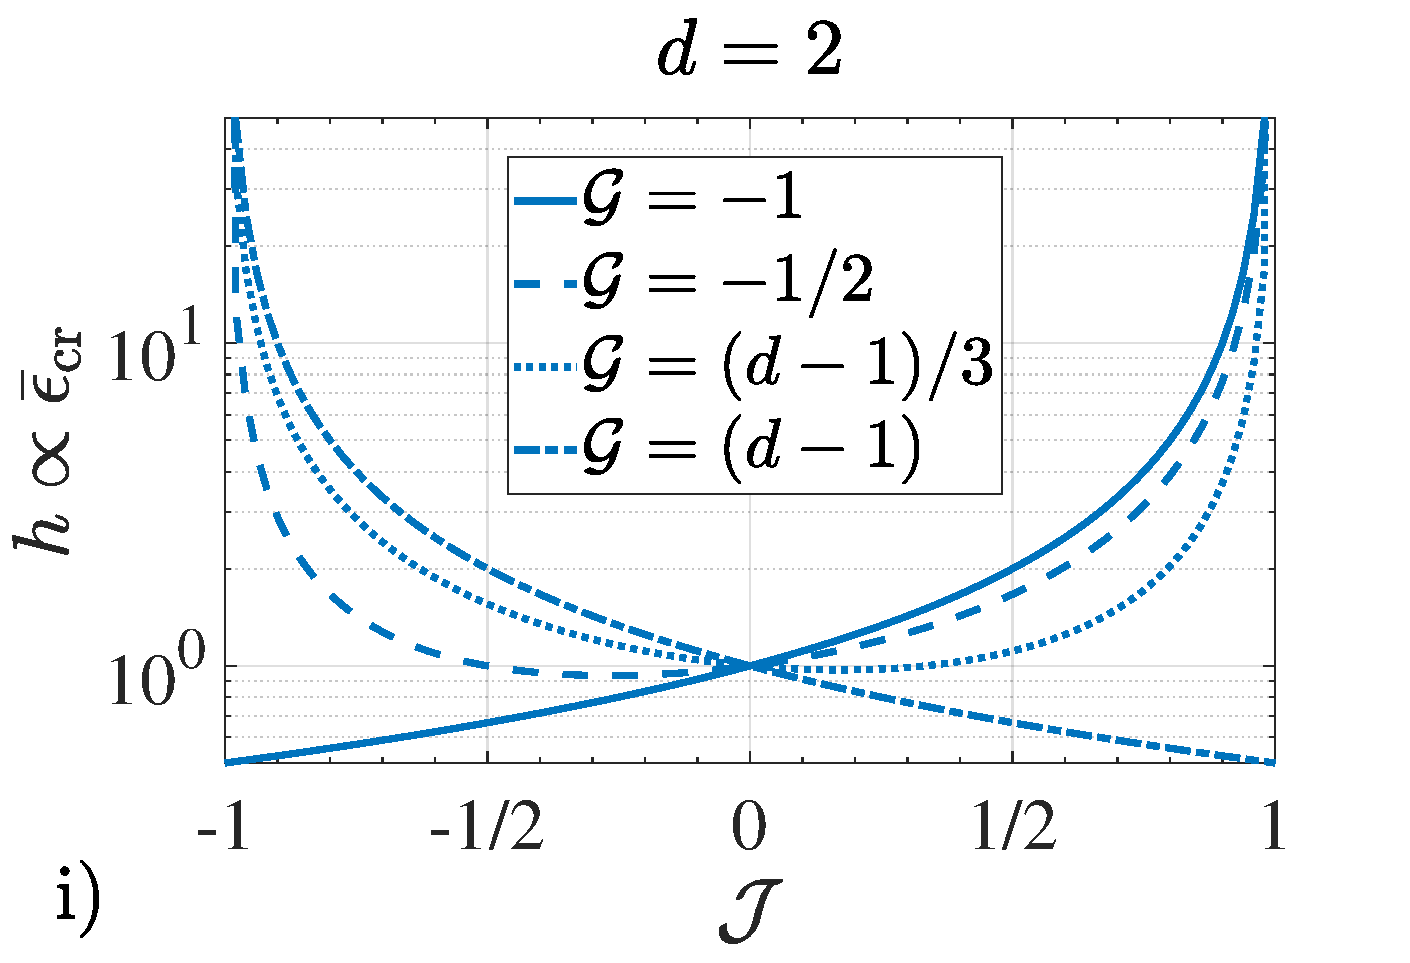
\includegraphics[trim={0cm 0.1cm 1.2cm 0cm},clip,width=7.75cm]{pictures/ch6_fig_extra_i}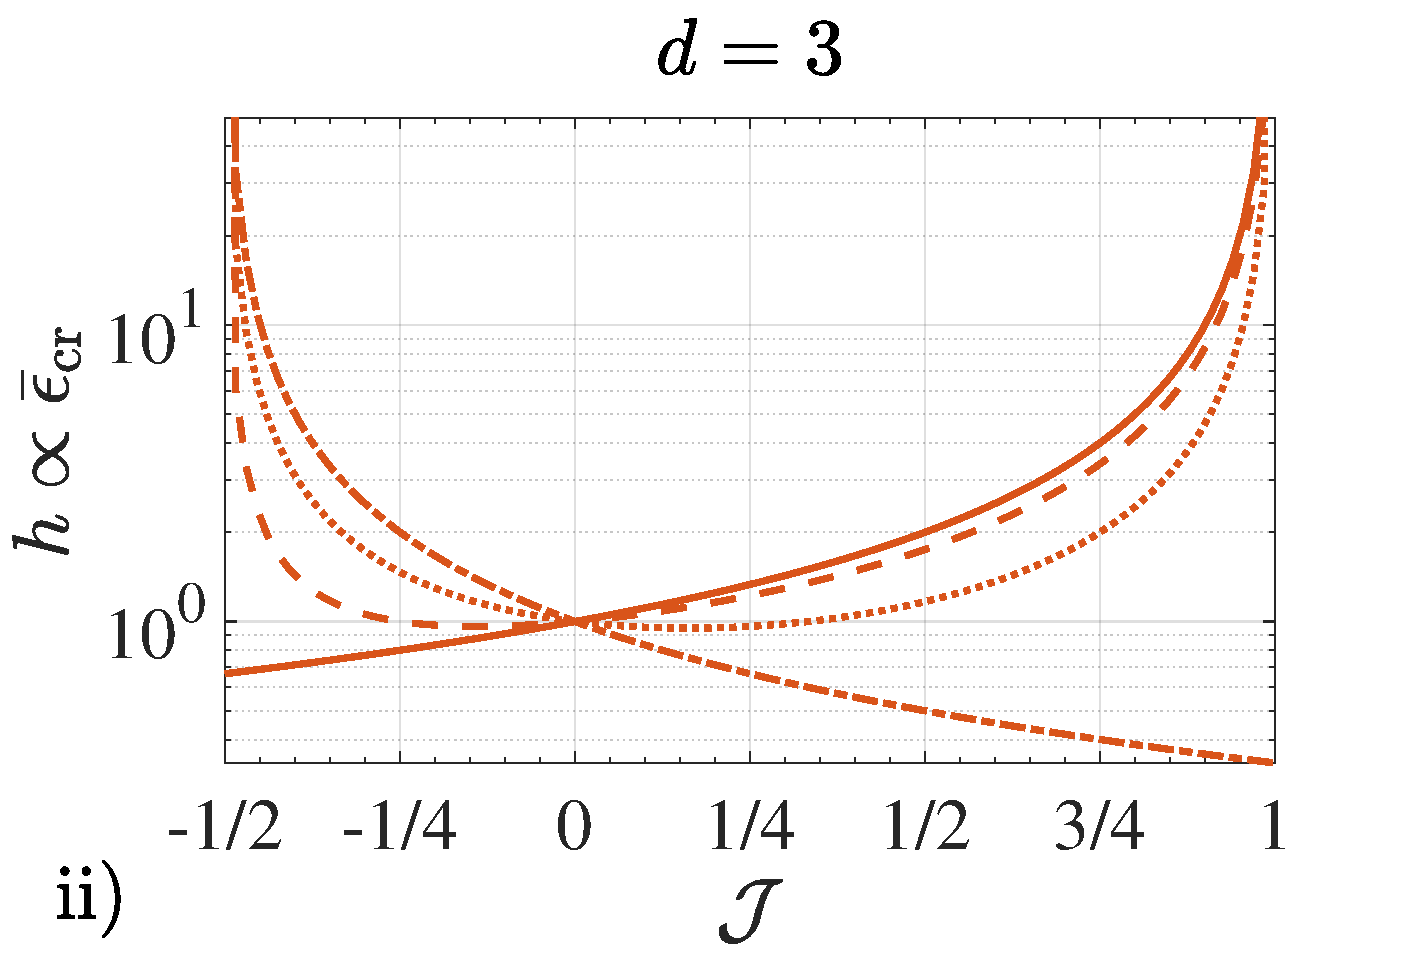
\includegraphics[trim={0cm 0.1cm 1.2cm 0cm},clip,width=7.75cm]{pictures/ch6_fig_extra_ii}
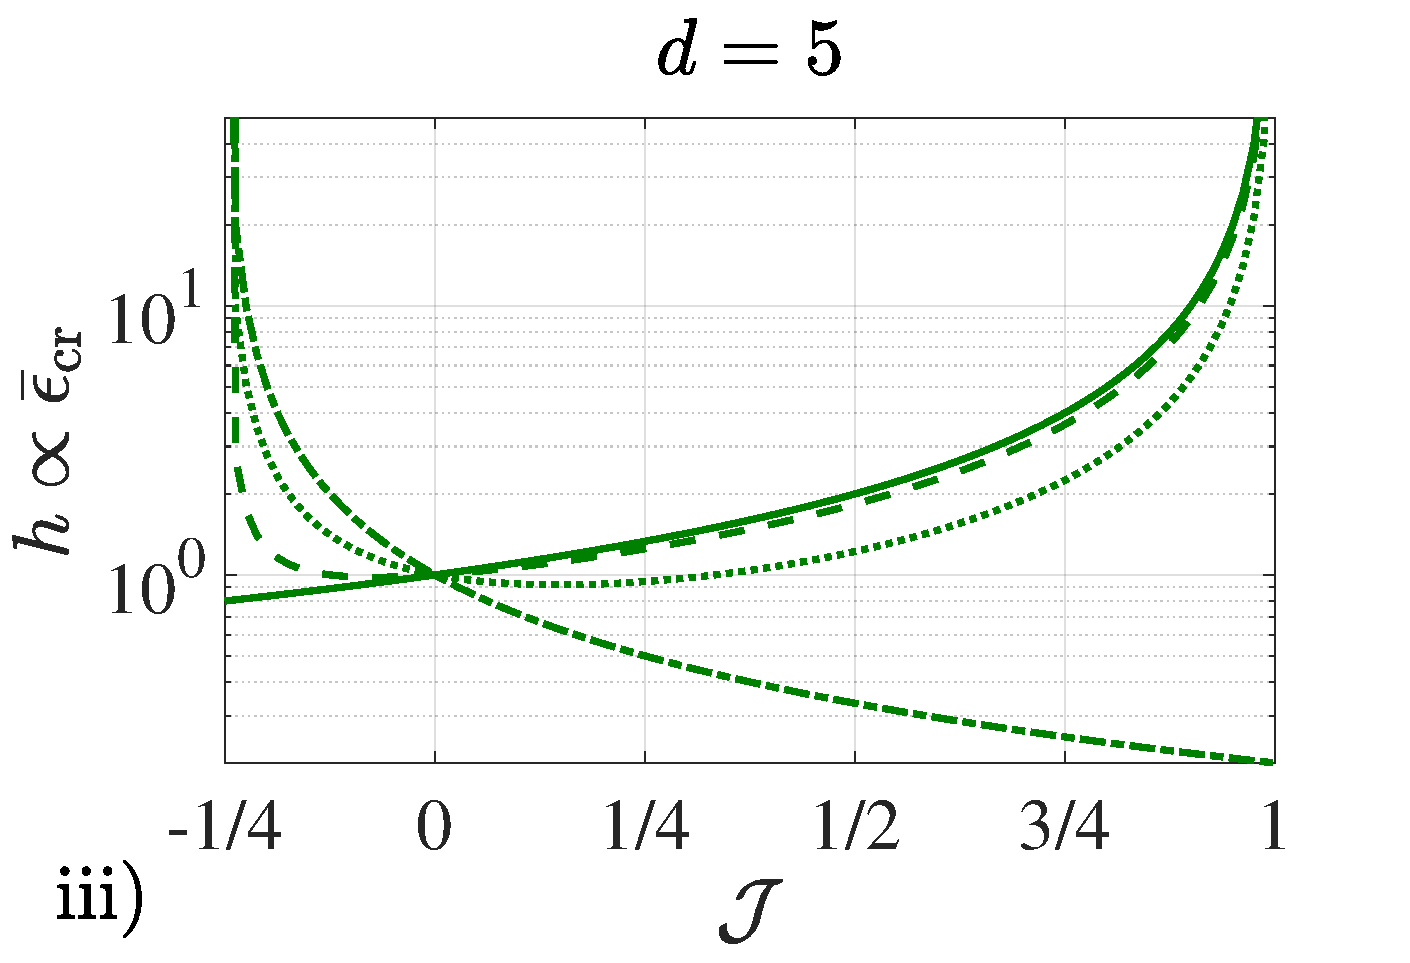
\includegraphics[trim={0cm 0.1cm 1.2cm 0cm},clip,width=7.75cm]{pictures/ch6_fig_extra_iii}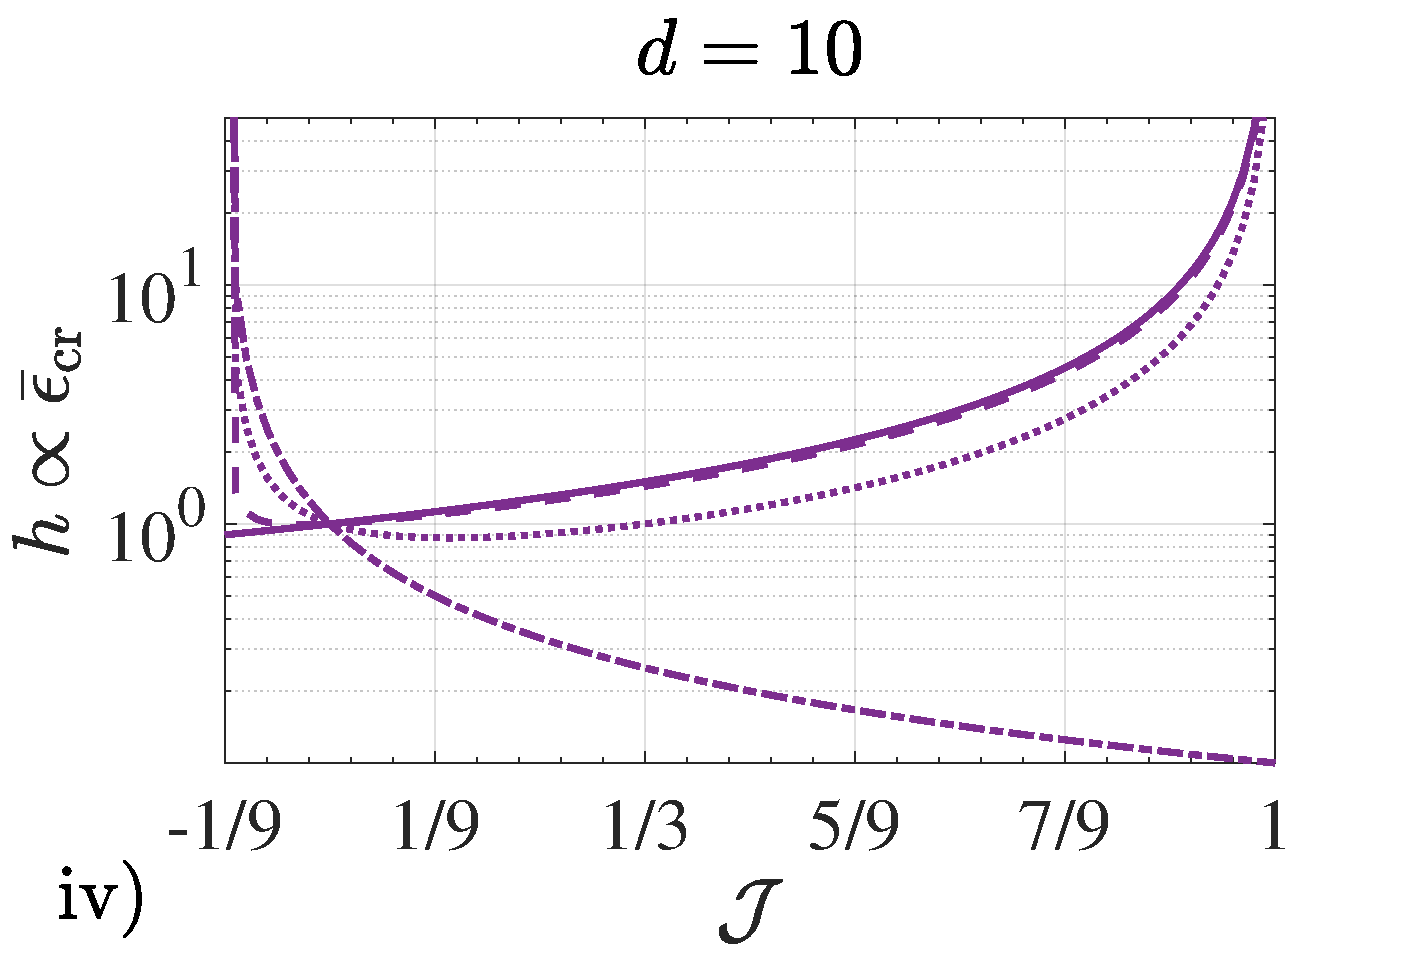
\includegraphics[trim={0cm 0.1cm 1.2cm 0cm},clip,width=7.75cm]{pictures/ch6_fig_extra_iv}
	\caption[Asymptotic uncertainty, correlations and geometry of the functions]{Representation of the interplay between the inter-sensor correlations $\mathcal{J}$ and the geometry parameter $\mathcal{G}$ in equation (\ref{geometrylinkfactor}) for a quantum sensing network with (i) $d=2$, (ii) $d=3$, (iii) $d=5$ and (iv) $d=10$ natural parameters. We observe that, given $\mathcal{G} \in (-1, (d-1))$, the minimum uncertainty is achieved using a scheme with inter-sensor correlations of strength $\mathcal{J} \in (1/(1-d),1)$. The quantitative characterisation of these minima is provided in section \ref{subsec:intersensorasymp}.}
\label{geolinkplot}
\end{figure}

\subsection{The role of inter-sensor correlations I: asymptotic case}
\label{subsec:intersensorasymp}

Let us exploit the previous result to address the problem of selecting an arrangement that is optimal to estimate a specific set of linear functions, which was introduced in section \ref{subsec:relevantinfo}. Mathematically, we need to find the values for $v$ and $\mathcal{J}$ that are optimal for a given $\mathcal{G}$. One approach is to use the fact that, for qubits, $0\leqslant 4v\leqslant 1$, which allows us to lower bound equation (\ref{symmetricfunctionssecond}) as $\bar{\epsilon}_{\mathrm{cr}} \geqslant \bar{\epsilon}_{\mathrm{f}} = \mathcal{N}h\left(\mathcal{J}, \mathcal{G}, d\right)/\mu$ and focus on searching for the amount of correlations $\mathcal{J}$ that minimises this bound after having fixed $\mathcal{G}$, $d$ and $\mu$. In principle, there is no guarantee that the pairs $(4v = 1, \mathcal{J})$ generated by this method will correspond to any physical state, although the bounds on the asymptotic error constructed in this way would still be valid. Nevertheless, later in this section we will study an example that can realise a large portion of the pairs $(4v = 1, \mathcal{J})$ that we are going to predict.

\begin{figure}[t]
\centering
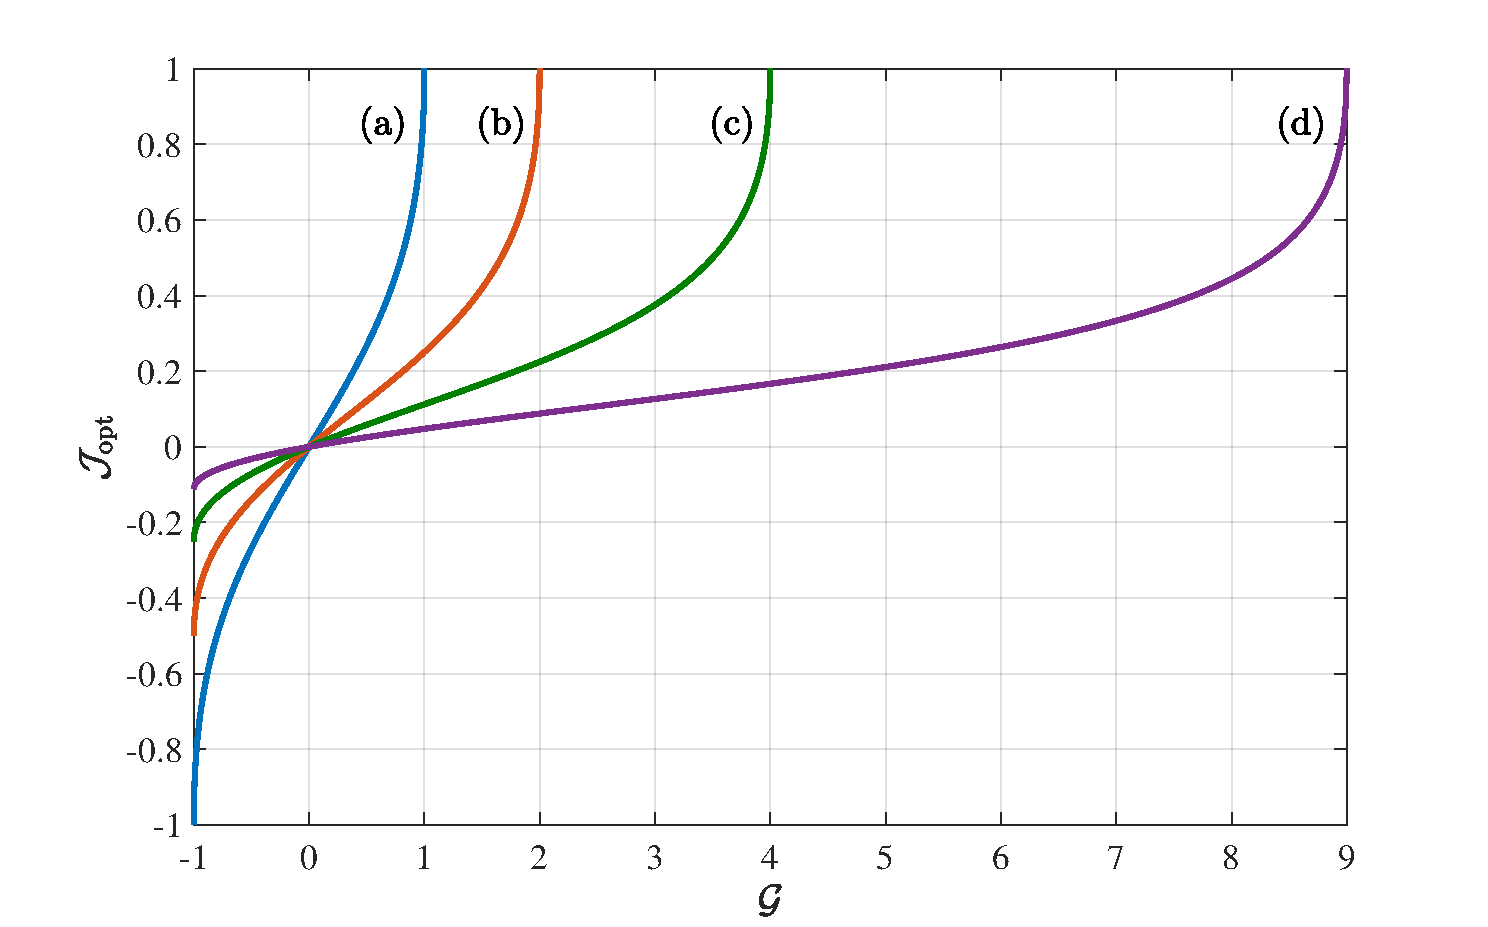
\includegraphics[trim={1cm 0.1cm 1.5cm 0.5cm},clip,width=14.75cm]{pictures/ch6_fig1}
	\caption[Optimal link between correlations and geometry of the functions]{Optimal link between the inter-sensor correlations $\mathcal{J}$ and the geometry $\mathcal{G}$ of a set of arbitrary linear functions, for $d=2$, $3$, $5$ and $10$. The analytical formula of this result has been provided in equation (\ref{optgeolinkanalytical}).}
\label{linkgeoent}
\end{figure}

The minimisation of $\bar{\epsilon}_{\mathrm{f}}$ reveals that, if $4v = 1$, and restricting our attention to the range $1/(1-d)<\mathcal{J} < 1$, the optimal strength for the inter-sensor correlations of the network is
\begin{equation}
\mathcal{J}_{\mathrm{opt}} = \frac{1}{\mathcal{G}+2-d}\left[1- \sqrt{\frac{(\mathcal{G}+1)(d-1-\mathcal{G})}{d-1}}\right],
\label{optgeolinkanalytical}
\end{equation}
for $-1 < \mathcal{G} < d-1$, which is determined by the structure of the functions alone via $\mathcal{G}$ once $d$ has been fixed\footnote{This result can be found as follows. If we look at $\bar{\epsilon}_{\mathrm{f}}$ as a function of $\mathcal{J}$, then the equation for its extrema is
\begin{equation}
\frac{\mathcal{N}}{\mu}\frac{\partial h\left(\mathcal{J}, \mathcal{G}, d\right)}{\partial \mathcal{J}} = \frac{\mathcal{N}}{\mu} \frac{(d-1)(d-2-\mathcal{G})\mathcal{J}^2+ 2(d-1)\mathcal{J} - \mathcal{G}}{(1 -\mathcal{J})^2[1+(d-1)\mathcal{J}]^2} = 0,
\nonumber
\label{slope}
\end{equation}
whose solutions are
\begin{equation}
\mathcal{J}_{\pm} = \frac{1}{\mathcal{G}+2-d}\left[1\mp \sqrt{\frac{(\mathcal{G}+1)(d-1-\mathcal{G})}{d-1}}\right].
\nonumber
\end{equation}
Since we need to restrict our study to the range $1/(1-d)<\mathcal{J} < 1$ for $F_q$ to be invertible, only $\mathcal{J_{+}}$ is a valid candidate to find a minimum. Next we examine the sign of the slope in the left hand side of equation (\ref{slope}) for some values of $\mathcal{J}$ around $\mathcal{J_{+}}$. By noticing that $\mathcal{N}/\mu > 0$ and using the endpoints of the domain for $\mathcal{J}$ we find that
\begin{equation}
\frac{\partial h\left(1 - \varepsilon, \mathcal{G}, d\right)}{\partial \mathcal{J}} > 0, ~~\frac{\partial h\left(1/(1-d) + \varepsilon, \mathcal{G}, d\right)}{\partial \mathcal{J}} < 0
\nonumber
\end{equation}
for an arbitrarily small $\varepsilon > 0$ when $\mathcal{G}\neq -1$, $\mathcal{G}\neq d-1$, which we exclude to guarantee that $\mathcal{J}\neq 1/(1-d)$, $\mathcal{J}\neq 1$. Consequently, $\mathcal{J_{+}}$ gives rise to the minimum that we were looking for.}. Crucially, equation (\ref{optgeolinkanalytical}) provides a map between correlations and geometry with one-to-one correspondence\footnote{Note that $\mathcal{J}_{\mathrm{opt}} \rightarrow (d-2)/[2(d-1)] $ when $\mathcal{G} \rightarrow d - 2$.}, as it can be directly verified in the representation of equation (\ref{optgeolinkanalytical}) in figure \ref{linkgeoent}. This is the central result of our asymptotic analysis.

Equation (\ref{optgeolinkanalytical}) reveals that, the more a collection of functions is clustered around the vector of ones $\boldsymbol{1}$, the larger the amount of positive correlations is required to be in order to perform the estimation optimally, provided that $4v=1$. Similarly, the amount of correlations with negative strength needs to be large if the functions are instead clustered around the subspace orthogonal to $\boldsymbol{1}$. The potential existence of this type of connection between geometry and correlations was precisely one of the general open questions identified by the authors of \cite{proctor2017networked}, which here has been answered in a definite way for the case of sensor-symmetric states. 

Furthermore, both equation (\ref{optgeolinkanalytical}) and figure \ref{linkgeoent} show that any amount of pairwise correlations would be detrimental whenever the geometry parameter vanishes. We need then to find out which kind of linear functions imply that $\mathcal{G} = 0$. To achieve this goal, let us recall our original definition for $\mathcal{G}$ in equation (\ref{geometryparameter}), that is, $\mathcal{G} = \mathrm{Tr}(\mathcal{W}_f V^\transpose \mathcal{X} V)/\mathcal{N}$. If we choose the uniform weighting matrix $\mathcal{W}_f = \mathbb{I}/l$ and $V$ is an orthogonal transformation, such that $VV^\transpose = V^\transpose V =  \mathbb{I}$, then 
\begin{equation}
\mathcal{G} = \frac{1}{\mathcal{N} l }\mathrm{Tr}(V V^\transpose \mathcal{X}) = \frac{1}{\mathcal{N} l}\mathrm{Tr}(\mathcal{X})=\frac{1}{\mathcal{N} l}  \mathrm{Tr}(\mathcal{I} - \mathbb{I})= 0.
\end{equation}
Now we observe that $\mathcal{J} = 0$, which is the optimal choice for the previous scenario, is always achieved by a separable qubit state $\ket{\psi_0} = (\sqrt{a}\ket{0} + \sqrt{1 - a}\ket{1})^{\otimes d}$, and by selecting $a = 1/2$ we have that $4v = 1$. Thus we can say that the estimation of a set of $l = d$ linear functions that are equally relevant and orthonormal can be carried out optimally by preparing our scheme with separable states. Moreover, since the estimation of the original parameters is a particular case of this type of transformation, our result implies that separable states are also sufficient for the optimal estimation of the primary properties. In other words, our formalism is consistent with the results available in the literature \cite{proctor2017networked, proctor2017networkedshort, altenburg2018, kok2017}. 

According to our definitions of \emph{local} and \emph{global} properties in section \ref{subsec:relevantinfo}, the previous conclusion is technically sufficient to affirm that while entangled pure states are generally useful for the optimal estimation of global properties, it is not true that we always need entangled probes in such case. However, a transformation that is orthogonal preserves angles and lengths, and for that reason one may argue that, in a sense, the information encoded by a set of functions that gives rise to an orthogonal transformation is equivalent to the information content of the original parameters, provided that the weighting matrices are uniform. Hence, it is perhaps not surprising that a local estimation strategy is preferred here, since Proctor \emph{et al.} \cite{proctor2017networked, proctor2017networkedshort} had already shown that the estimation of local properties associated with commuting generators can be performed optimally with a local strategy. 

In view of this, it is desirable to establish whether there are global properties with $\mathcal{G} = 0$ that select information that is not equivalent to estimate all the original parameters. First we observe that the eigendecomposition of $\mathcal{X}$, which is a symmetric matrix, is
\begin{equation}
\mathcal{X}_D = U_{\mathcal{X}}^\transpose \mathcal{X} U_{\mathcal{X}} = \mathrm{diag}\left[(d-1), -1, \dots, -1 \right], 
\end{equation} 
where the eigenvector for the first eigenvalue is $\boldsymbol{1}$ and those for the other eigenvalues belong to the orthogonal subspace\footnote{The characteristic equation for $\mathcal{X}$ is 
\begin{equation}
\mathrm{det}\left(\mathcal{X} - \lambda\mathbb{I}\right) = \mathrm{det}\left[\boldsymbol{1}\boldsymbol{1}^\transpose - (1 + \lambda)\mathbb{I}\right] \propto \left(1 - d + \lambda\right)\left(1+\lambda\right)^{d-1} = 0, 
\nonumber
\end{equation}
giving the eigenvalues $\lambda_1 = d-1$, with multiplicity $1$, and $\lambda_2 = -1$, with multiplicity $d-1$ (see the calculation for equation (\ref{characteristicfim}), which is formally similar to the one here). By inspection we see that $\boldsymbol{1}$ is one of the eigenvectors. Since the latter satisfies that $\mathcal{X}\boldsymbol{1} = (\boldsymbol{1}\boldsymbol{1}^\transpose - \mathbb{I})\boldsymbol{1} = (d-1)\boldsymbol{1}$, the rest of the eigenvalues must be associated with the subspace orthogonal to $\boldsymbol{1}$, and this concludes the eigendecomposition of $\mathcal{X}$.}. That implies that if we choose a single linear function as $V = \boldsymbol{f} = U_{\mathcal{X}}\boldsymbol{1}$, then we will have that $\mathcal{G} = \boldsymbol{1}^\transpose U_{\mathcal{X}}^\transpose \mathcal{X} U_{\mathcal{X}} \boldsymbol{1}/d = \boldsymbol{1}^\transpose \mathcal{X}_D \boldsymbol{1}/d=0$. Imagine that we consider a three-parameter network, so that 
\begin{eqnarray}
\boldsymbol{f} = U_{\mathcal{X}}\boldsymbol{1} = \frac{1}{\sqrt{6}}
\begin{pmatrix}
\sqrt{2} & \sqrt{3} & 1\\
\sqrt{2} & -\sqrt{3} & 1\\
\sqrt{2} & 0 & -2\\
\end{pmatrix} 
\begin{pmatrix}
1 \\
1 \\
1 \\
\end{pmatrix} 
= \frac{1}{\sqrt{6}}
\begin{pmatrix}
\sqrt{2} + \sqrt{3} + 1 \\
\sqrt{2} - \sqrt{3} + 1 \\
\sqrt{2} -2 \\
\end{pmatrix}.
\end{eqnarray}
Clearly, this is a global property, and, as a consequence, this result strengthens the idea that entanglement is sometimes not needed in scenarios where we are estimating global properties. Interestingly, the same argument fails for $d=2$, since in that case
\begin{equation}
\boldsymbol{f} = U_{\mathcal{X}}\boldsymbol{1} = \frac{1}{\sqrt{2}}
\begin{pmatrix}
1 & 1 \\
1 & -1
\end{pmatrix}
\begin{pmatrix}
1 \\
1
\end{pmatrix} =
\begin{pmatrix}
\sqrt{2} \\
0
\end{pmatrix},
\end{equation}
which simply rescales the first parameter, and this is a local property. Nonetheless, our conclusion above is still valid in general.

For the link between geometry and correlations in equation (\ref{optgeolinkanalytical}) to be truly useful, it is necessary that there are physical states with the properties that such link predicts as optimal. Consider first a network where $d=2$. Proctor \emph{et al.} (appendix E of \cite{proctor2017networked}) studied the estimation of $1 \leqslant l \leqslant d$ linear and normalised but otherwise arbitrary functions using the sensor-symmetric state 
\begin{equation}
\ket{\psi_0} = \frac{1}{\sqrt{2\left(1+\gamma^2\right)}}\left[\ket{0 0} + \gamma\left(\ket{01} + \ket{10}  \right) + \ket{1 1}\right],
\label{gammastatetwo}
\end{equation}
with $-\infty < \gamma < \infty$, which is a particular case of the more general formalism that we are developing in this chapter. The fact that the authors of \cite{proctor2017networked} succeeded in solving their problem completely with this state suggests that the latter may realise all the pairs $(4v = 1, \mathcal{J})$ that are optimal according to our results.

Recalling that $\sigma_z \ket{i} = (-1)^{i}\ket{i}$, we can see that, for the state in equation (\ref{gammastatetwo}), $\langle \sigma_{z,1} \rangle = \langle \sigma_{z,2} \rangle = 0$ and $\langle \sigma_{z,1} \sigma_{z,2} \rangle = \langle \sigma_{z,1} \sigma_{z,2} \rangle = (1-\gamma^2)/(1+\gamma^2)$, so that the variance is $4v = 4v_1 = 4v_2 = 1$ and the quantifier for the inter-sensor correlations can be written as a function of $\gamma$ as $\mathcal{J}=(1-\gamma^2)/(1+\gamma^2)$. This function reaches the maximum $\mathcal{J}=1$ at $\gamma = 0$, while it tends monotonically from such point to $\mathcal{J} = - 1$ when $\gamma \rightarrow \pm \infty$. In other words, for $d=2$ there is always a physical state that satisfies the condition imposed in equation (\ref{optgeolinkanalytical}) when $4v = 1$.

It is interesting to observe that $\gamma$ splits the state in a part where the sum of the parameters is encoded and a part that can encode the difference. More concretely\footnote{For this calculation we have used that
\begin{equation}
\mathrm{e}^{i\varphi\sigma_z}\ket{j} = \sum_{k=1}^\infty \frac{\left(i\varphi\right)^k}{k!} \sigma_z^k\ket{j} = \sum_{k=1}^\infty \frac{\left(i\varphi\right)^k}{k!} (-1)^{jk}\ket{j} = \mathrm{e}^{i(-1)^j \varphi}\ket{j}.
\nonumber
\end{equation}},
\begin{align}
\mathrm{e}^{-\frac{i}{2}(\sigma_{z,1}\theta_1+\sigma_{z,2}\theta_2)}\ket{\psi_0} = &~ \frac{1}{\sqrt{2\left(1+\gamma^2\right)}}\left[\mathrm{e}^{-\frac{i}{2}(\theta_1 + \theta_2)}\ket{0 0} + \mathrm{e}^{\frac{i}{2}(\theta_1 + \theta_2)}\ket{1 1} \right] 
\nonumber \\
&+ \frac{\gamma}{\sqrt{2\left(1+\gamma^2\right)}}\left[\mathrm{e}^{-\frac{i}{2}(\theta_1 - \theta_2)}\ket{01} + \mathrm{e}^{\frac{i}{2}(\theta_1 - \theta_2)}\ket{10} \right].
\label{twonetworktransformed}
\end{align}
A partial extension of this idea to the $d$-parameter case can be achieved by constructing a state where the part that encodes functions aligned with the direction of $\boldsymbol{1}$ is separated in an analogous fashion, i.e., 
\begin{eqnarray}
\ket{\psi_0} &=& \frac{1}{\sqrt{2\left[1 + \left( 2^{d-1}-1 \right)\gamma^2 \right]}} \left[\left(1-\gamma\right)\left(\ket{0}^{\otimes d} + \ket{1}^{\otimes d}\right) + \gamma \left(\ket{0} + \ket{1} \right)^{\otimes d} \right].
\nonumber \\
&\propto& \ket{0 0 \dots 0} + \ket{1 1 \dots 1} + \gamma \left(\text{the rest of the terms}\right).
\label{gammastategen}
\end{eqnarray}
For this probe, $4v_i = 1 - \langle \sigma_{z,i} \rangle^2 = 1  = 4v$ for all $i$, and $4c_{ij} = \langle \sigma_{z,i} \sigma_{z,j} \rangle - \langle \sigma_{z,i} \rangle\langle \sigma_{z,j} \rangle = \langle \sigma_{z,i} \sigma_{z,j} \rangle = (1-\gamma^2)/[1 + (2^{d-1}-1)\gamma^2] = 4c$ for all $i\neq j$, verifying in this way that the state in equation (\ref{gammastategen}) is also sensor symmetric. As a result, we can see that its inter-sensor correlations are given by
\begin{equation}
\mathcal{J} = \frac{1-\gamma^2}{1 + \left(2^{d-1}-1\right)\gamma^2}.
\label{gengammacorrelations}
\end{equation} 
If $0 \leqslant \abs{\gamma} \leqslant 1$, then we have that $1 \geqslant \mathcal{J} \geqslant 0$. This implies that there always exists a physical state associated with all the results in this section that require either positive inter-sensor correlations, or the absence of them. On the other hand, the amount of negative correlations that this state can cover lies in $ 0 > \mathcal{J} > - 1/(2^{d-1}-1)$, which corresponds to $1 < \abs{\gamma} < \infty$. Unfortunately, the amount of negative correlations that equation (\ref{optgeolinkanalytical}) might predict can lie in $ 0 > \mathcal{J} > 1/(1-d)$, where $1/(1-d) \leqslant - 1/(2^{d-1}-1)$ for $d\geqslant 2$ and the inequality is only saturated when $d=2$. Thus there is a subinterval not covered by equation (\ref{gammastategen}). Whether there are other physical states that may realise the missing values is an open question. 

Finally, we draw attention to the fact that the only entangled pure probes that may be asymptotically relevant for sensor-symmetric networks are those that give rise to inter-sensor correlations, while any other form of entanglement will be irrelevant in this type of scenario. To illustrate this idea, let us consider the state in equation (\ref{gammastategen}) for $d = 3$, and suppose that the functions to be estimated are associated with $\mathcal{G} = 0$. We have seen that, in that case, no inter-sensor correlations are needed to perform the estimation optimally, which implies that, according to equation (\ref{gengammacorrelations}), $\gamma = \pm 1$ . By inserting these parameters in equation (\ref{gammastategen}) we find that the optimal states are
\begin{equation}
\ket{\psi_{+}} = \frac{1}{2\sqrt{2}}\left(\ket{0}+\ket{1}\right)^{\otimes 3}
\end{equation}
and
\begin{equation}
\ket{\psi_{-}} = \frac{1}{2\sqrt{2}} \left[2\left(\ket{0}^{\otimes 3} + \ket{1}^{\otimes 3}\right) - \left(\ket{0} + \ket{1} \right)^{\otimes 3} \right].
\end{equation}
The first state is separable, but it can be shown that $\ket{\psi_{-}}$ is not. If we tried to write the latter as
$\ket{\psi_{-}} = (x_0\ket{0}+x_1\ket{1})(y_0\ket{0}+y_1\ket{1})(z_0\ket{0}+z_1\ket{1})$, with $|x_0|^2+|x_1|^2 = |y_0|^2+|y_1|^2  = |z_0|^2+|z_1|^2 = 1$, we would find contradictions such as 
\begin{equation}
\left[(x_0 = x_1) \land (x_0 = - x_1)\right]\land (|x_0|^2+|x_1|^2 = 1),
\end{equation}
which by \emph{reductio ad absurdum} allows us to conclude that the state with $\gamma = -1$ and $d = 3$ is entangled. Hence, while here entanglement is not required to reach the asymptotic optimum, neither is it necessarily detrimental. The only requirement imposed by our formalism is the absence of pairwise correlations, and the presence or absence of any other kind of correlation does not affect the uncertainty. 

\subsection{Multi-parameter prior information analysis}
\label{subsec:multiprioranalysis}

Now we focus on two-parameter networks and we turn to the more general problem of estimating linear functions when different amounts of data are available, using our findings about the properties of the asymptotically optimal quantum probes as a guide. To do this, our prior knowledge needs to be consistent with the idea that, if we were to keep repeating the experiment, our scheme would continue being useful (section \ref{theory}). In other words, our prior must allow for the asymptotic regime to be reached, which requires a multi-parameter analysis of the prior information.

In section \ref{subsec:multinonasym} we concluded that a suitable prior for this problem in the regime of moderate prior knowledge is the multi-parameter flat density in equation (\ref{multiprior}). Since our network is highly symmetric, it is appropriate to imagine that our prior information is similar for both parameters, and this justifies assuming that $W_{0,i} = W_0$ and $\bar{\theta}_i = \bar{\theta}$ for $i = 1 , 2$, where we recall that $W_{0, i}$ and $\bar{\theta}_i$ were the prior width and the prior mean for the $i$-th primary parameter. Hence, the prior area is simply $\Delta_0 = W_0^2$, and we will choose $\bar{\theta} = W_0/2$ for the Bayesian calculations in this chapter. 

Next we need to choose $W_0$ (and thus the prior area $\Delta_0$) such that the likelihood does not contain ambiguous information in the region where the original parameters can lie, and to construct the likelihood we have to select a measurement. As with the state, we wish to select an asymptotically optimal POM, which is achieved by requiring that $F(\boldsymbol{\theta})=F_q$. We know that a POM fulfilling this condition always exists for the scenario with pure states and commuting generators considered here (\cite{sammy2016compatibility, pezze2017simultaneous} and sections \ref{subsec:crb} and \ref{subsec:multiasymp}), since, in such case, the symmetric logarithmic derivatives are not unique and we may find some pair of logarithmic derivatives that commute, which would allow us to construct the POM \cite{sammy2016compatibility}. Alternatively, Humphreys \emph{et al.} \cite{humphreys2013} proposed a set of projectors such that one of the elements is the original state, while the rest are orthogonal to it, and this idea was refined and extended in \cite{pezze2017simultaneous} by identifying conditions that projective POMs need to fulfil to have that $F(\boldsymbol{\theta})=F_q$. However, for us it suffices to follow a simpler approach; first we will provide a qualitative argument suggesting a potential measurement scheme, and then we will verify that it is indeed optimal by a direct calculation.  

Although we wish to estimate functions, the condition $F(\boldsymbol{\theta})=F_q$ refers only to the original parameters, and we know that these can be estimated optimally using a local strategy (\cite{proctor2017networked, proctor2017networkedshort} and section \ref{subsec:intersensorasymp}). In view of this, a local POM might be sufficient to make the classical and quantum information matrices equal, and, in fact, this would be very useful for our analysis, since in that case we could associate any enhancement derived from the presence of correlations with the initial state. 

Consider then the local POM $\ket{n, k} = \left[\ket{0} + (-1)^n \ket{1}\right]\otimes[\ket{0} + (-1)^k \ket{1}]/2$, for $n, k = 0, 1$. In addition, we have seen that, if $d=2$, then the state in equation (\ref{gammastatetwo}) is sufficient to realise all the asymptotic results predicted by our theory. As such, we will use this probe for our Bayesian calculation. Combining this POM with the transformed state $\ket{\psi(\theta_1, \theta_1)} = \mathrm{e}^{-\frac{i}{2}(\sigma_{z,1}\theta_1+\sigma_{z,2}\theta_2)}\ket{\psi_0}$ in equation (\ref{twonetworktransformed}), the probability amplitude is
\begin{align}
\braket{n,k}{\psi(\theta_1, \theta_2)}  \propto &~ \mathrm{e}^{-\frac{i}{2}(\theta_1+\theta_2)} + (-1)^{n+k}\mathrm{e}^{\frac{i}{2}(\theta_1+\theta_2)}
\nonumber \\
&+\gamma\left[(-1)^k \mathrm{e}^{-\frac{i}{2}(\theta_1-\theta_2)} + (-1)^n \mathrm{e}^{\frac{i}{2}(\theta_1-\theta_2)}\right]
\nonumber \\
\propto &~ \mathrm{cos}\left\lbrace\left[\theta_1 + \theta_2 + \pi(k+n)\right]/2\right\rbrace
\nonumber \\
&+ \gamma\hspace{0.15em}\mathrm{cos}\left\lbrace\left[\theta_1 - \theta_2 - \pi(k-n)\right]/2\right\rbrace,
\end{align}
the modulus of the proportionality factor being $1/\sqrt{2(1+\gamma^2)}$. This allows us to find the likelihood function
\begin{equation}
p(n, k | \theta_1, \theta_2) = ||\braket{n,k}{\psi(\theta_1, \theta_2)}||^2 = \left[\mathrm{cos}(x_{+}) + \gamma \mathrm{cos}(x_{-})\right]^2/[2(1+\gamma^2)],
\label{multilikelihood}
\end{equation}
where we have introduced the notation $x_{\pm} \equiv \left[\theta_1 \pm \theta_2 \pm \pi(k\pm n)\right]/2$.

The elements of the classical Fisher information matrix for the probability in equation (\ref{multilikelihood}) are
\begin{align}
[F(\boldsymbol{\theta})]_{11} &= \sum_{n,k = 0}^1 \frac{1}{p(n, k | \theta_1, \theta_2)}\left[\frac{\partial p(n, k | \theta_1, \theta_2)}{\partial \theta_1} \right]^2 
\nonumber \\
&= \frac{1}{2\left(1+\gamma^2 \right)} \sum_{n,k = 0}^1  \left[ \mathrm{sin}(x_{+}) + \gamma \mathrm{sin}(x_{-}) \right]^2 = 1,
\label{classfimqubit1}
\end{align}
\begin{align}
[F(\boldsymbol{\theta})]_{22} &= \sum_{n,k = 0}^1 \frac{1}{p(n, k | \theta_1, \theta_2)}\left[\frac{\partial p(n, k | \theta_1, \theta_2)}{\partial \theta_2} \right]^2 
\nonumber \\
&= \frac{1}{2\left(1+\gamma^2 \right)} \sum_{n,k = 0}^1 \left[ \mathrm{sin}(x_{+}) - \gamma \mathrm{sin}(x_{-}) \right]^2 = 1,
\end{align}
and
\begin{align}
[F(\boldsymbol{\theta})]_{12} &= \sum_{n,k = 0}^1 \frac{1}{p(n, k | \theta_1, \theta_2)}\frac{\partial p(n, k | \theta_1, \theta_2)}{\partial \theta_1}\frac{\partial p(n, k | \theta_1, \theta_2)}{\partial \theta_2} 
\nonumber \\
&= \frac{1}{2\left(1+\gamma^2 \right)} \sum_{n,k = 0}^1 \left[ \mathrm{sin}^2(x_{+}) - \gamma^2 \mathrm{sin}^2(x_{-})  \right] = \frac{1-\gamma^2}{1+\gamma^2},
\label{classfimqubit3}
\end{align}
with $[F(\boldsymbol{\theta})]_{21}= [F(\boldsymbol{\theta})]_{12}$. On the other hand, in sections \ref{sec:networksasym} and \ref{subsec:intersensorasymp} (see also appendix E of \cite{proctor2017networked}) we have seen that, for this configuration,
\begin{equation}
F_q = 
\begin{pmatrix}
1 & \mathcal{J} \\
\mathcal{J} & 1
\end{pmatrix} =
\begin{pmatrix}
1 & (1-\gamma^2)/(1+\gamma^2) \\
(1-\gamma^2)/(1+\gamma^2) & 1
\end{pmatrix},
\end{equation}
which is identical to the classical Fisher information matrix in equations (\ref{classfimqubit1} - \ref{classfimqubit3}). Therefore, we conclude that the quantum strategy formed by the previous local POM and the state in equation (\ref{gammastatetwo}) is asymptotically optimal. 

Following section \ref{subsec:multinonasym}, one way of identifying the size of the region where the likelihood function of this strategy is free of ambiguities is to represent the posterior probability $p(\theta_1, \theta_2|\boldsymbol{n}, \boldsymbol{k}) \propto p(\boldsymbol{n}, \boldsymbol{k} |\theta_1, \theta_2)$, where $\boldsymbol{n} = (n_1, \dots, n_\mu)$ and $\boldsymbol{k} = (k_1, \dots, k_\mu)$, so that we can visualise the regions with an asymptotically unique absolute maximum in a direct fashion. The result of this operation, which is based on the algorithm in appendix \ref{sec:multiprior}, is shown in figure \ref{priornetwork} for several values of $\gamma$. 

\begin{figure}[t]
\centering
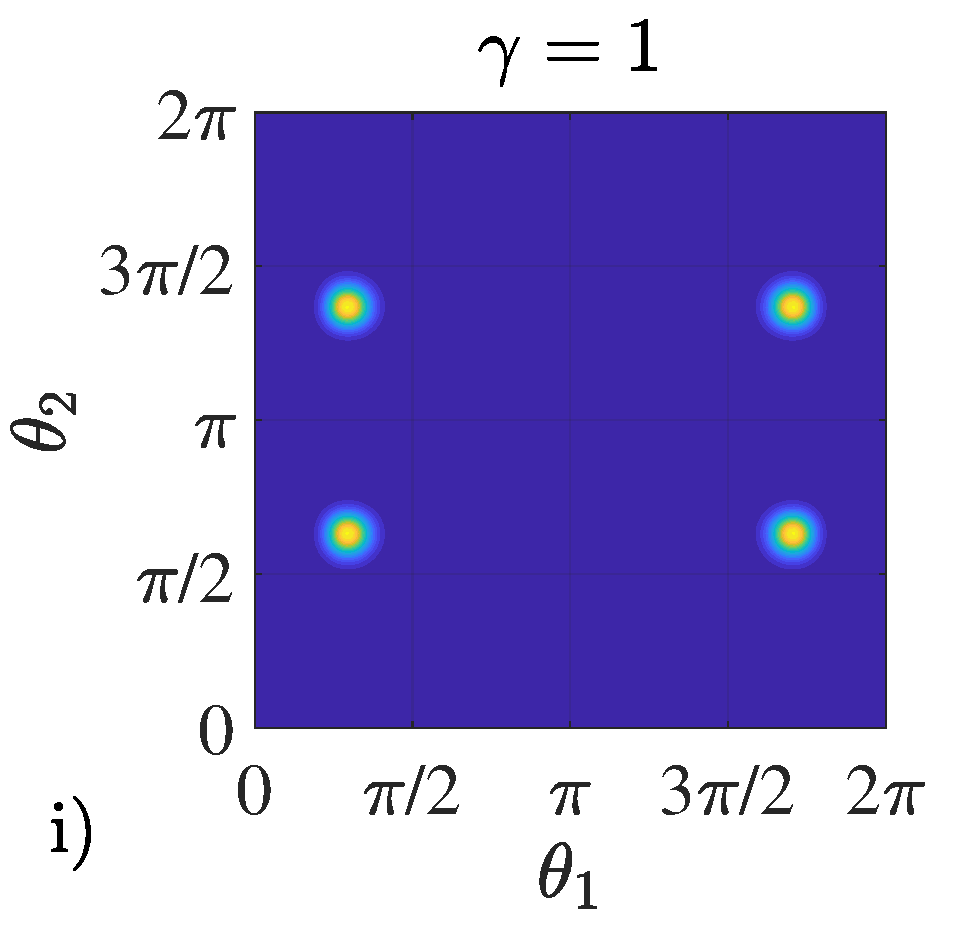
\includegraphics[trim={0.2cm 0cm 0.5cm 0cm},clip,width=5.1cm]{ch6_fig2i}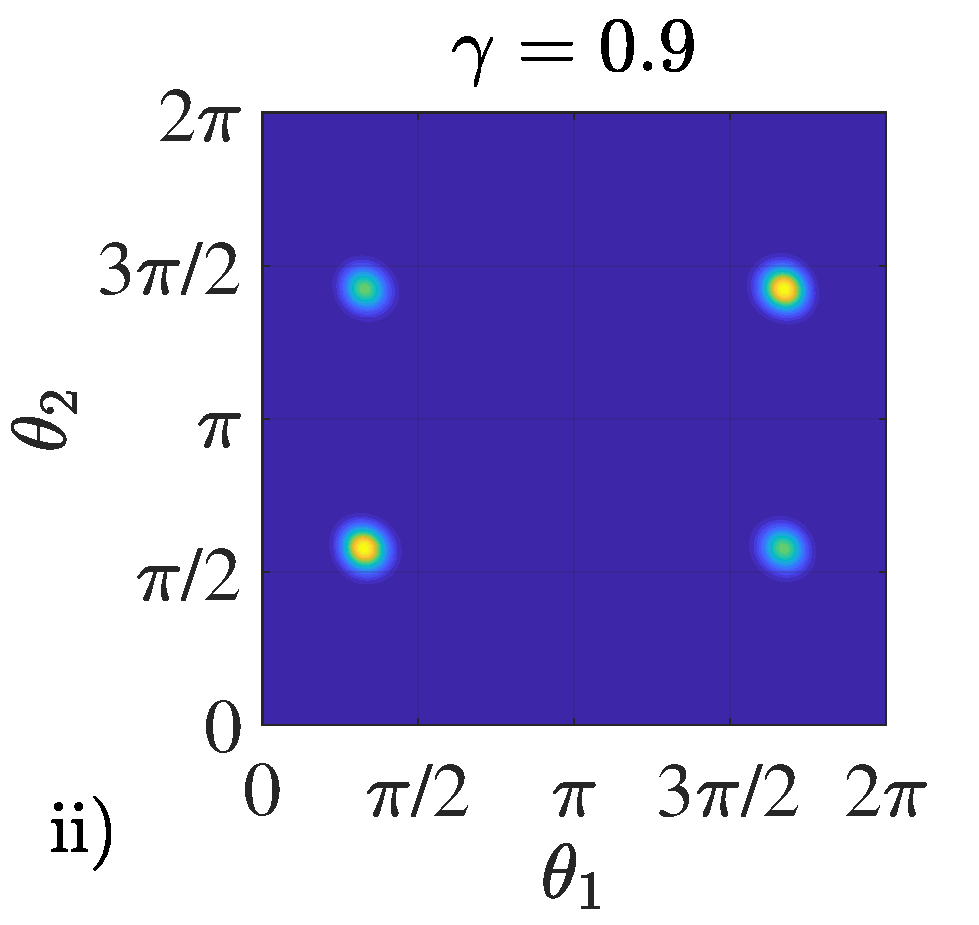
\includegraphics[trim={0.2cm 0cm 0.5cm 0cm},clip,width=5.1cm]{ch6_fig2ii}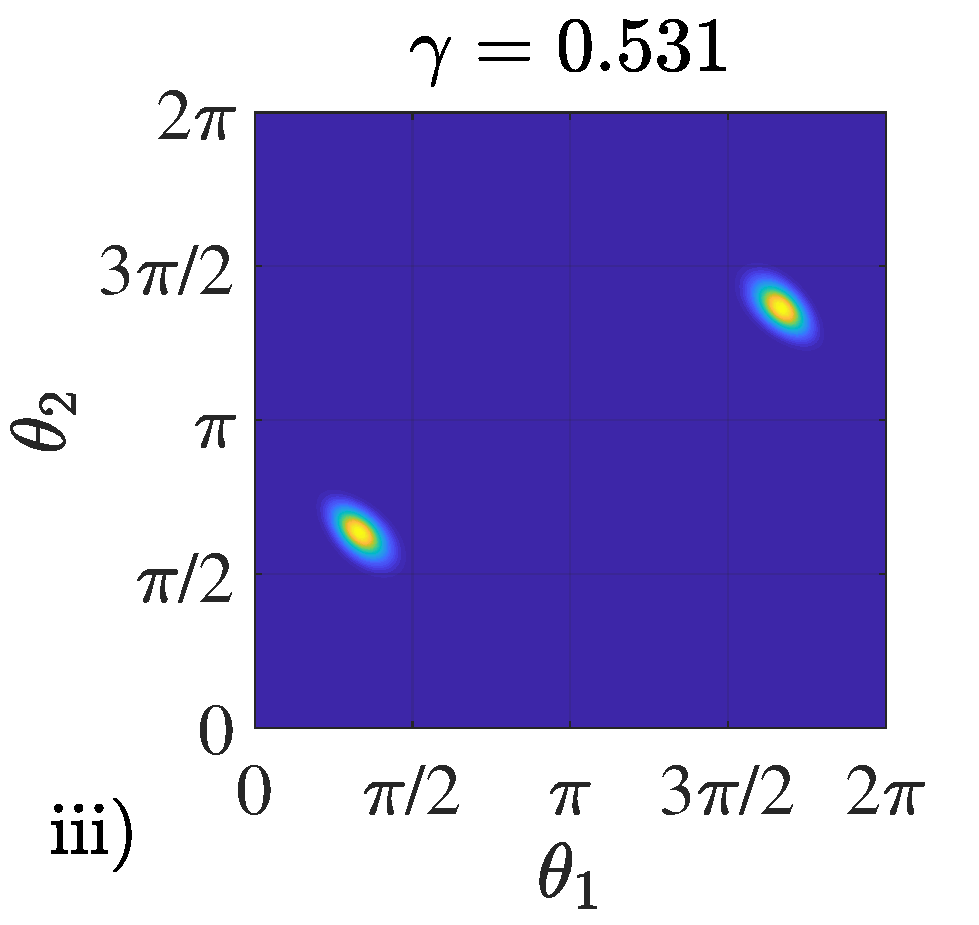
\includegraphics[trim={0.2cm 0cm 0.5cm 0cm},clip,width=5.1cm]{ch6_fig2iii}
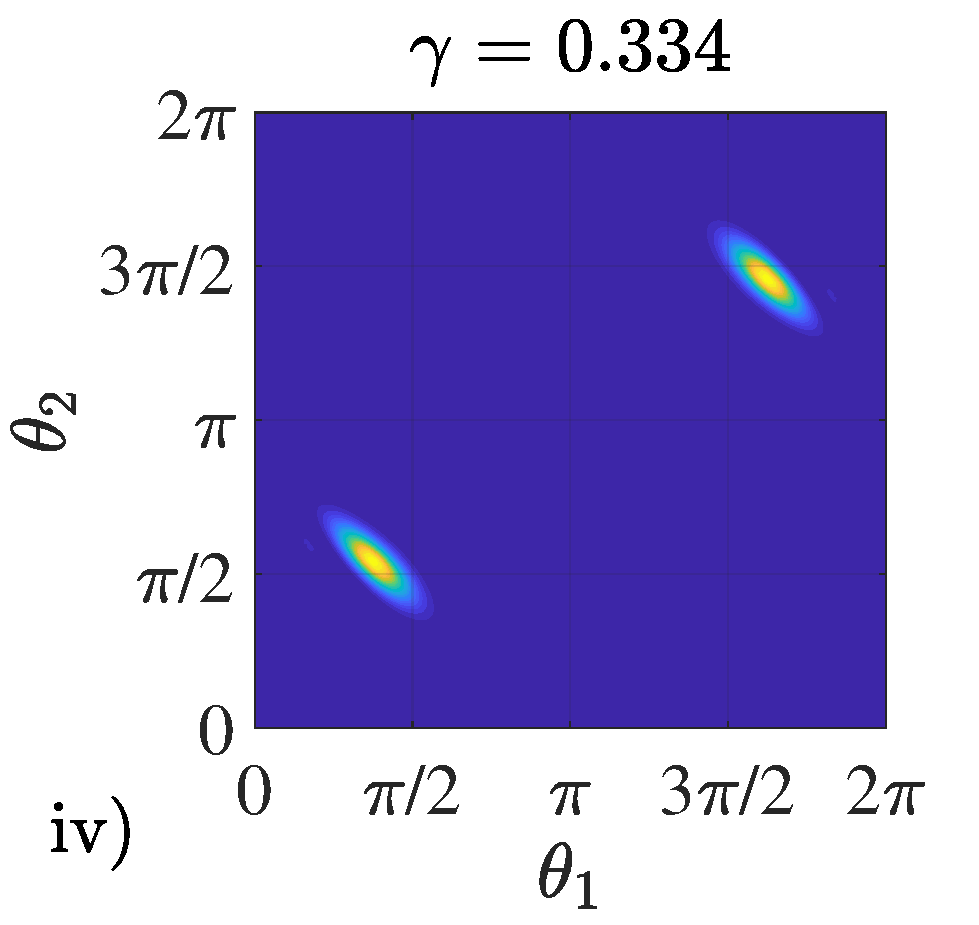
\includegraphics[trim={0.2cm 0cm 0.5cm 0cm},clip,width=5.1cm]{ch6_fig2iv}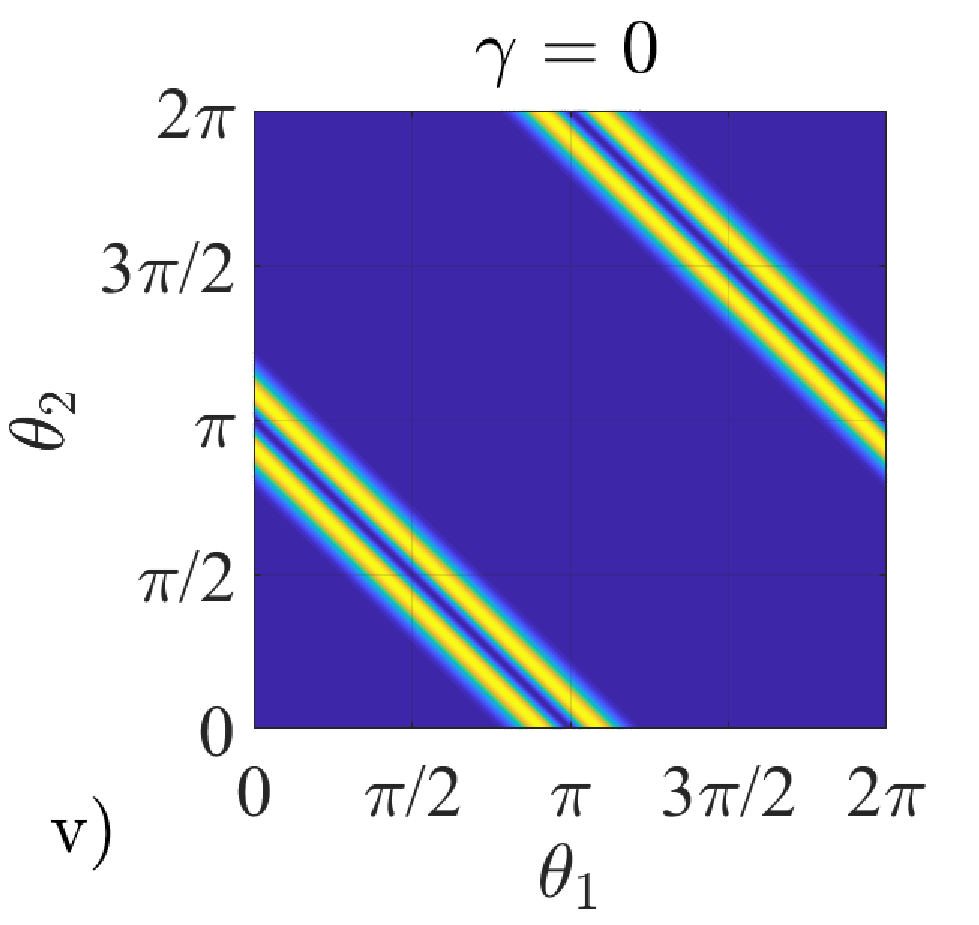
\includegraphics[trim={0.1cm 0cm 0.5cm 0cm},clip,width=5.1cm]{ch6_fig2v}
\caption[Prior information analysis of a two-parameter scheme]{Posterior density functions for random simulations of $\mu = 100$ trials, a flat prior and the quantum strategy represented by the likelihood in equation (\ref{multilikelihood}), with (i) $\gamma = 1$, (ii) $\gamma = 0.9$, (iii) $\gamma = 0.531$, (iv) $\gamma = 0.334$ and (v) $\gamma = 0$. The simulated true values of the original parameters are $\theta'_1=1$ and $\theta'_2=2$. We draw attention to the fact that the representation for $1 < \gamma < \infty $ follows the same pattern but with the posterior peaks tending to the direction orthogonal to that in (v).}
\label{priornetwork}
\end{figure}

First we note that the simulations in figure \ref{priornetwork} have been restricted to the area $(\theta_1, \theta_2) \in [0, 2\pi]\times [0, 2\pi]$ because it is clear that the single-shot likelihood in equation (\ref{multilikelihood}) is invariant under   $\theta_i \rightarrow \theta_i + 2\pi m$, with $m = 0, \pm 1, \pm 2, \dots$ and $i=1,2$\footnote{The calculations required to arrive at this conclusion are analogous to those in section \ref{subsec:prioranalysis} for the NOON state.}, and thus it suffices to examine the symmetries within one period. While the number of maxima changes with $\gamma$, we can observe that all the ambiguities in figures \ref{priornetwork}.i - \ref{priornetwork}.iv can be avoided if the prior area satisfies that $\Delta_0 = W_0^2 \leqslant \pi^2$. 

The situation for $\gamma = 0$ in figure \ref{priornetwork}.v is, however, different. In that case, no single peak can be selected even after a large number of repetitions, which implies that such scheme does not have an asymptotic approximation. This is consistent with the fact that, if $\gamma = 0$, then $\mathcal{J} = 1$, and according to our results in section \ref{sec:networksasym}, this case needs to be excluded for the Fisher information matrix to be invertible. Furthermore, the same type of behaviour would have been observed if we had examined the limit $|\gamma| \rightarrow \infty$, for which $\mathcal{J}\rightarrow -1$. Hence, we only need to impose the existence of a unique maximum for $0 < |\gamma| < \infty$. As such, we conclude that, given our configuration, the intrinsic area is $\Delta_\mathrm{int} = W_\mathrm{int}^2 = \pi^2$, provided that the parameters are thought of as independent before the experiment is performed.

Crucially, the previous discussion does not imply that the scheme with $\gamma = 0$ is useless. Figure \ref{priornetwork}.v shows   that this scheme is giving information about the combination $\theta_2 + \theta_1 = \pi m$, with $m = 0, \pm 1, \pm 2, \dots$, that is, about the sum of the parameters. In fact, this can be seen in a very transparent way by inserting $\gamma = 0$ in equation (\ref{multilikelihood}), since then the likelihood for a single shot is only sensitive to the sum of the primary parameters. The calculations in the next section will reveal that while the performance of this scheme is generally poor in the asymptotic regime, it can be useful when $\mu$ is low.

\subsection{The role of inter-sensor correlations II: non-asymptotic case}
\label{subsec:correlationsmultibayes}

Using the quantum strategy in section \ref{subsec:multiprioranalysis} for a two-sensor qubit network  and the optimal estimator found in section \ref{subsec:multiasymp}, we wish to estimate two global properties of such network when the experiment operates both in and out of the regime of limited data. In particular, we consider the linear functions $f_1(\boldsymbol{\theta}) = (2\theta_1 + \pi \theta_2)/\sqrt{4+\pi^2}$ and $f_2(\boldsymbol{\theta}) = (2\theta_1 + \theta_2)/\sqrt{5}$, which we encode in the columns of $V$ as
\begin{equation}
V = \frac{1}{\sqrt{20 + 5\pi^2}}
\begin{pmatrix}
2\sqrt{5} & 2\sqrt{4+\pi^2}\\
\pi \sqrt{5} & \sqrt{4+\pi^2}
\end{pmatrix}.
\label{funlimiteddata}
\end{equation}
To complete this task, we assume that both functions are equally relevant, so that $\mathcal{W}_f = \mathbb{I}/2$, and that our prior knowledge is represented by the prior probability $p(\theta_1, \theta_2) = 4/\pi^2$, when $(\theta_1, \theta_2) \in [0, \pi/2]\times[0, \pi/2]$, and zero otherwise. Since $\Delta_0 = \pi^2/4 < \pi^2 = \Delta_\mathrm{int}$, our analysis in section \ref{subsec:multiprioranalysis} implies that this prior assignment will allow us to reach the asymptotic regime.

Let us start by comparing a local strategy with an entangled scheme that is asymptotically optimal. The former assumes that the experiment is arranged such that $\gamma = 1$, $\mathcal{J} = 0$, while to find the properties of the latter we need to recall our results in section \ref{subsec:intersensorasymp} for the asymptotic role of inter-sensor correlations. Equation (\ref{optgeolinkanalytical}) indicates that, for $d = 2$, 
\begin{equation}
\mathcal{J}_{\mathrm{opt}} = \left(1- \sqrt{1 - \mathcal{G}^2}\right)/\mathcal{G},
\label{twoparametergeolink}
\end{equation}
when $\mathcal{G}\neq 0$, and $\mathcal{J}_{\mathrm{opt}} = 0$ if $\mathcal{G} = 0$. In addition, $\mathcal{J} = (1-\gamma^2)/(1+\gamma^2)$, and by combining the latter expression with equation (\ref{twoparametergeolink}) we find that
\begin{equation}
\gamma_{\mathrm{opt}} = \pm \left(\frac{\mathcal{G}-1+\sqrt{1-\mathcal{G}^2}}{\mathcal{G} + 1 - \sqrt{1-\mathcal{G}^2}}\right)^{\frac{1}{2}},
\label{gammaoptlink}
\end{equation}
when $\mathcal{G}\neq 0$, and $\mathcal{\gamma}_{\mathrm{opt}} = 1$ if $\mathcal{G} = 0$. The normalisation term for the functions in equation (\ref{funlimiteddata}) is simply $\mathcal{N} = \mathrm{Tr}(\mathcal{W}_f V^\transpose V) = 1$, while the geometry parameter is $\mathcal{G} = \mathrm{Tr}\left(\mathcal{W}_f V^\transpose \mathcal{X} V \right)/\mathcal{N} = (8 + 10\pi + 2\pi^2)/(20 + 5\pi^2) \approx 0.853$, and by inserting this result in equations (\ref{twoparametergeolink}) and (\ref{gammaoptlink}) we have that $\gamma_\mathrm{opt} \approx \pm 0.531$ (we can choose the positive solution without loss of generality) and that $\mathcal{J} = 0.561$, where the latter verifies that this state is indeed entangled\footnote{This is because the two-sensor state in equation (\ref{gammastatetwo}) is only separable when $\gamma^2 = 1$. To show it, we just need to impose that
\begin{equation}
\left(x_0 \ket{0} + x_1\ket{1}\right)\left(y_0 \ket{0} + y_1\ket{1}\right) \propto \ket{00} + \gamma \left(\ket{01} + \ket{10} \right) + \ket{11},
\nonumber 
\end{equation}
from where the previous statement follows.}.   

\begin{figure}[t]
\centering
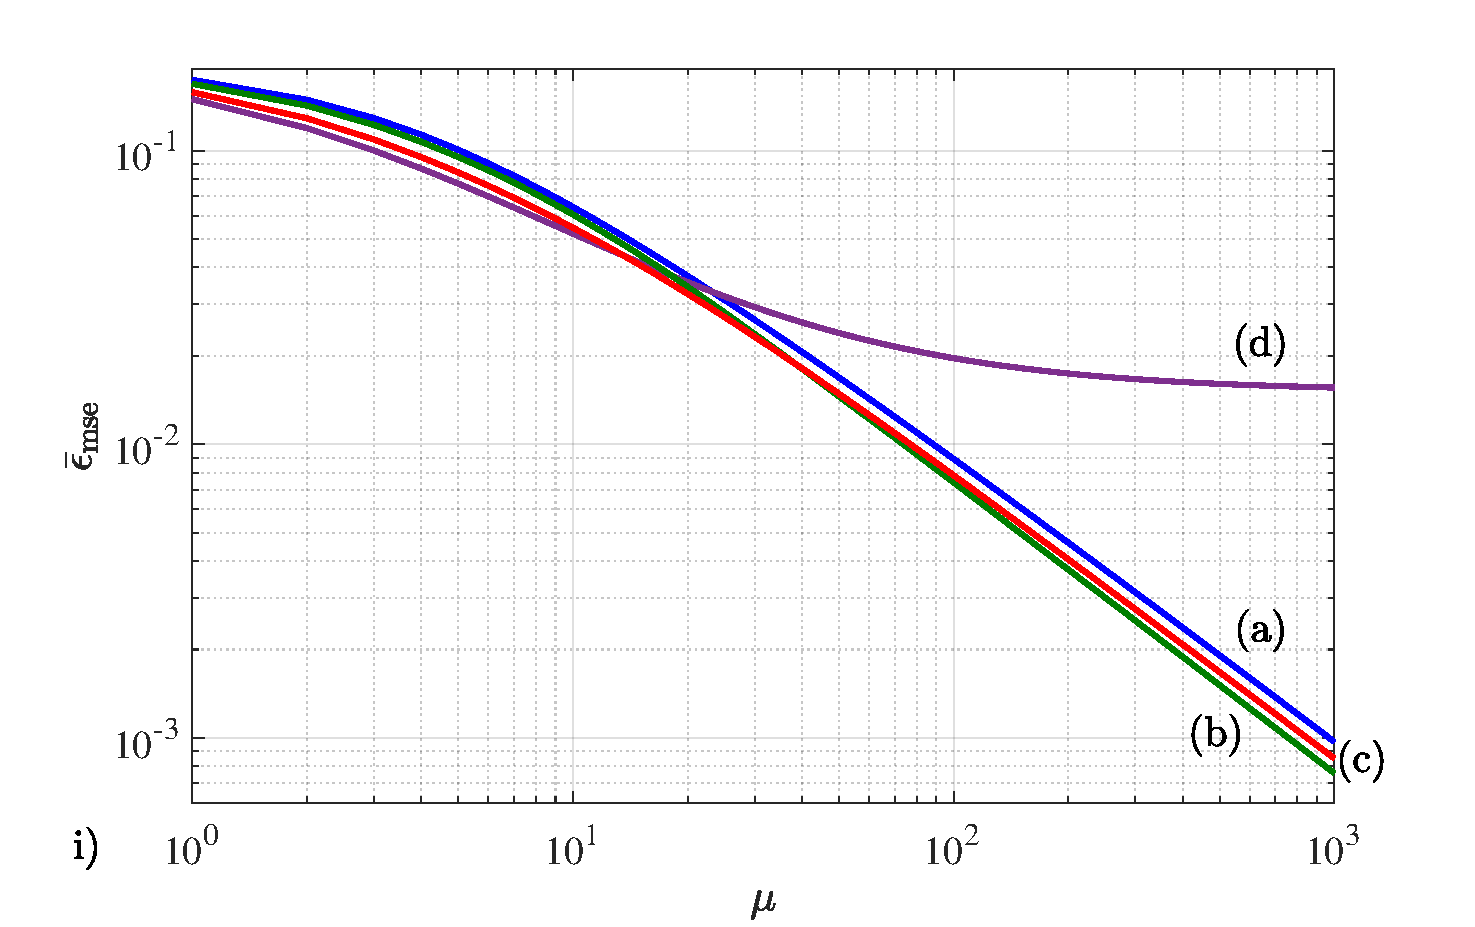
\includegraphics[trim={0.2cm 0cm 0.5cm 0cm},clip,width=14.75cm]{ch6_fig3i}
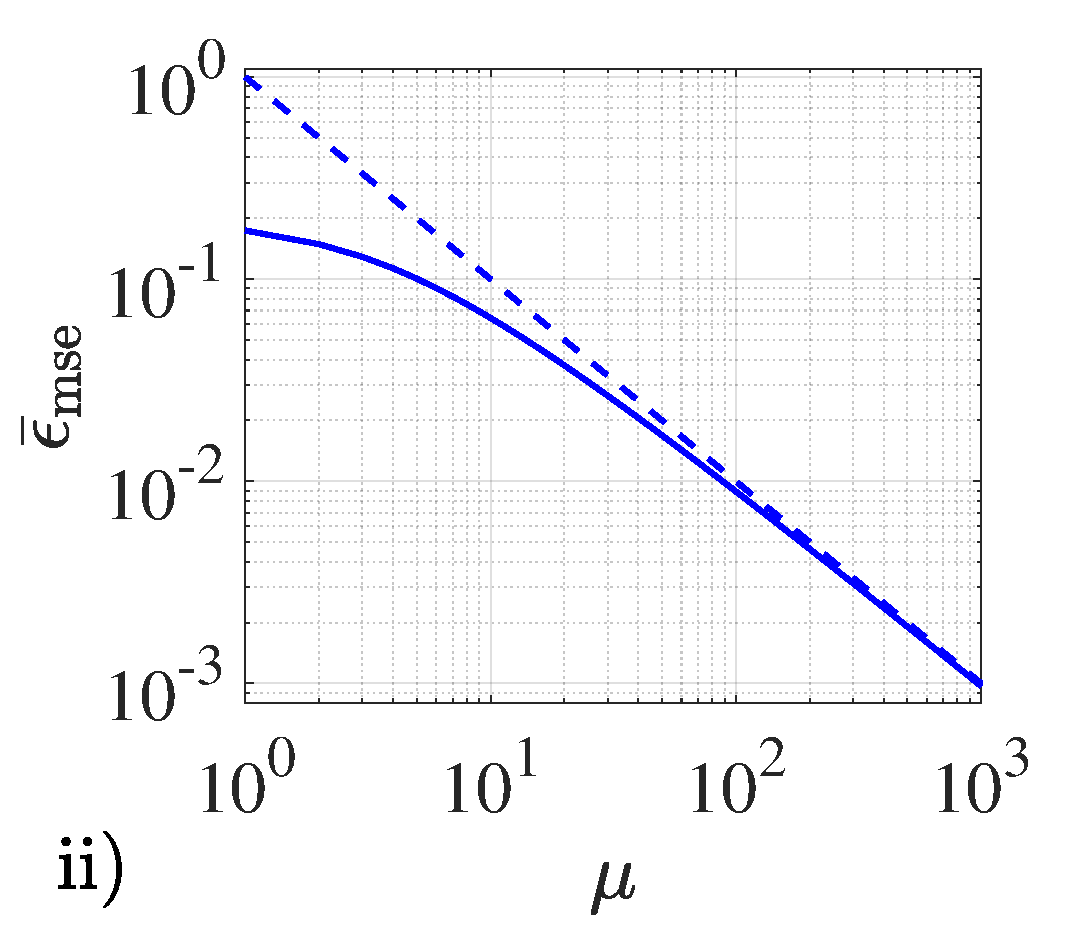
\includegraphics[trim={0.2cm 0cm 0.5cm 0cm},clip,width=5.1cm]{ch6_fig3ii}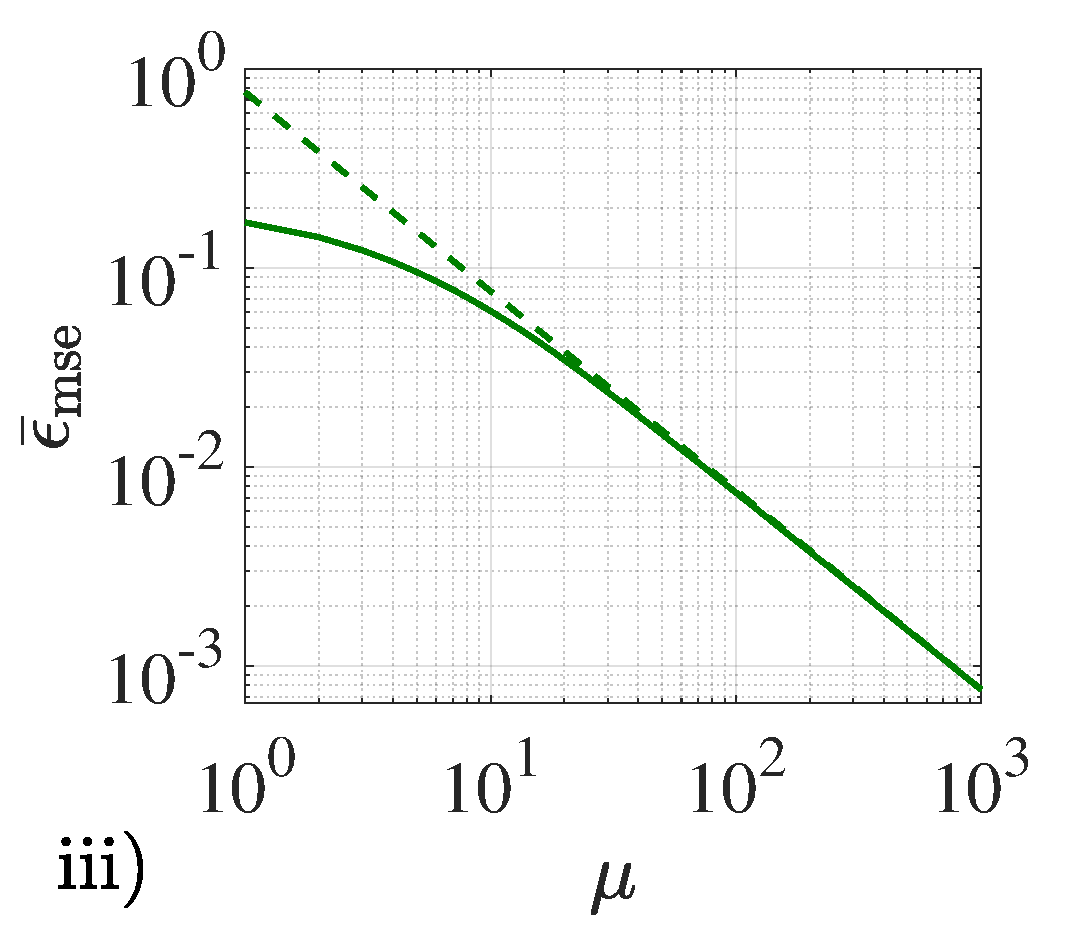
\includegraphics[trim={0.2cm 0cm 0.5cm 0cm},clip,width=5.1cm]{ch6_fig3iii}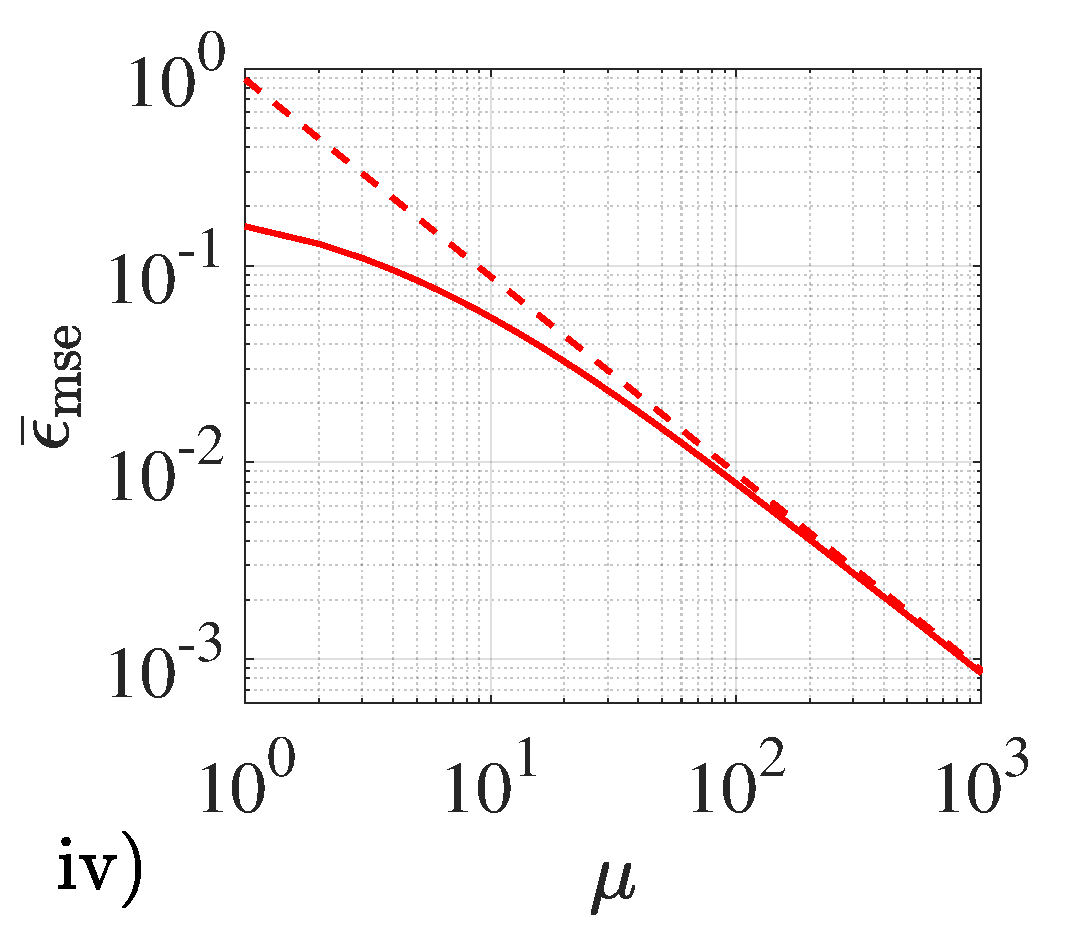
\includegraphics[trim={0.2cm 0cm 0.5cm 0cm},clip,width=5.1cm]{ch6_fig3iv}
\caption[Estimation of two linear functions in the non-asymptotic regime]{i) Mean square error for the estimation of the linear functions $f_1(\boldsymbol{\theta}) = (2\theta_1 + \pi \theta_2)/\sqrt{4+\pi^2}$ and $f_2(\boldsymbol{\theta}) = (2\theta_1 + \theta_2)/\sqrt{5}$ by means of the two-sensor qubit network introduced in section \ref{subsec:multiprioranalysis}, where (a) is a local strategy, with $\gamma = 1$, $\mathcal{J} = 0$; (b) is the asymptotically optimal entangled strategy, with $\gamma = 0.531$, $\mathcal{J} = 0.561$; (c) is a strategy whose enhancement has been balanced between the asymptotic and non-asymptotic regimes, with $\gamma = 0.334$, $\mathcal{J} = 0.799$; and (d) is a maximally entangled state, with $\gamma = 0$, $\mathcal{J} = 1$, while figures (ii - iv) compare the mean square error (solid lines) and the multi-parameter quantum Cram\'{e}r-Rao bound (dashed lines) for the strategies in (a - c). All the calculations assume the weighting matrix $\mathcal{W}_f = \mathbb{I}/2$ and a flat prior  of area $\Delta_0 = \pi^2/4$ and centred around $(\pi/4, \pi/4)$.}
\label{nonasymptoticnetwork}
\end{figure}

The numerical calculation of $\bar{\epsilon}_{\mathrm{mse}}$ in equation (\ref{msefunctionsmin}) for these two strategies can be performed with the algorithm in appendix \ref{sec:multimsematlab}, and the results have been represented in figure \ref{nonasymptoticnetwork}.i as graphs (a) for the local scheme and (b) for the optimal entangled strategy. We can observe that the local strategy performs worse than the entangled one for any number of repetitions. Therefore, in this case we have that the prediction made by the asymptotic theory is qualitatively preserved in the non-asymptotic regime. However, a closer analysis reveals that the distance between both graphs is considerably shorter when $1 \leqslant \mu \lesssim 20$ than when $\mu \gg 1$. This behaviour is reminiscent of what we found for a Mach-Zehnder interferometer in figure \ref{bounds_results}.i, where some of the probes with a large Fisher information (and thus with a good asymptotic performance) had an error very close to that of a coherent laser beam in the regime of limited data, the latter being an optical analogue of the notion of local strategy in this chapter. Moreover, from the optical study we learned that a better asymptotic error was sometimes associated with a worse performance in the regime of low $\mu$. As a consequence, a natural question is whether we could obtain an uncertainty that is lower than the error for the asymptotically optimal entangled state when the network operates in the non-asymptotic regime. 

\begin{table} [t]
\centering
{\renewcommand{\arraystretch}{1.2}
\begin{tabular}{|l|c|c|c|}
\hline
Strategy & $\gamma$ & $\mathcal{J}$ & $\mu_{\tau} (\Delta_0=\pi^2/4)$ \\
\hline
\hline
Local & $1$ & $0$ & $4.58\cdot 10^2$ \\
Asymptotically optimal & $0.531$ &$0.561$ & $4.3\cdot 10$ \\
Balanced enhancement & $0.334$ & $0.799$ & $5.37\cdot 10^2$  \\
Maximally entangled & $0$ & $1$ & $-$ \\
\hline
\end{tabular}}
\caption[Bayesian study of a quantum sensing network]{Properties of different strategies based on a two-parameter qubit network, where $\gamma$ selects the state and $\mathcal{J}$ is the amount of inter-sensor correlations. Furthermore, the third column provides the number of repetitions needed such that the relative error between the Bayesian uncertainty and the Cram\'{e}r-Rao bound is equal to or less than $5\%$ (that is, $\varepsilon_\tau = 0.05$ in equation (\ref{saturation})). These results demonstrate the state-dependent nature of the conditions required to approach the Cram\'{e}r-Rao in multi-parameter systems.}
\label{multinetworkstable}
\end{table}

To test this idea, let us select a third arrangement with an asymptotic error that lies between those of the local scheme and the asymptotically optimal strategy. The asymptotic error for our network can be written in terms of $\gamma$ as (see equations (\ref{symmetricfunctionssecond}) and (\ref{geometrylinkfactor}))
\begin{equation}
\bar{\epsilon}_\mathrm{mse} \approx \bar{\epsilon}_{\mathrm{cr}} = \frac{\left(1+\gamma^2\right)\left[\left(1-\mathcal{G}\right)+\left(1+\mathcal{G}\right)\gamma^2\right]}{4\mu \gamma^2} \equiv \bar{\epsilon}_{\mathrm{qbit}}\left(\gamma\right),
\label{crmsetwoqubitnetwork}
\end{equation}
and using this we can find the $\gamma$ of the strategy satisfying our desideratum above by imposing that
\begin{equation}
\bar{\epsilon}_{\mathrm{qbit}}\left(\gamma\right) = \frac{1}{2}\left[\bar{\epsilon}_{\mathrm{qbit}}\left(\gamma_{\mathrm{loc}}=0\right) + \bar{\epsilon}_{\mathrm{qbit}}\left(\gamma_{\mathrm{ent}}=0.531\right)\right].
\end{equation}
The solutions of this equation are $\gamma \approx \pm 0.334 , \pm 0.842$, and we take our third strategy to be prepared such that $\gamma = 0.334$, $\mathcal{J} = 0.799$, since this is the option with the lowest uncertainty for a single shot\footnote{In particular, $\bar{\epsilon}_{\mathrm{mse}}(\mu = 1, \gamma = 0.334) \approx 0.158$ and $\bar{\epsilon}_{\mathrm{mse}}(\mu = 1, \gamma = 0.842) \approx 0.173$.}. 

The uncertainty $\bar{\epsilon}_{\mathrm{mse}}$ for the third scheme has been represented as a function of the number of trials in figure \ref{nonasymptoticnetwork}.i, where it is labelled as (c). As expected, this error lies between the local and the asymptotically optimal strategies when $\mu \gg 1$, but this is no longer the case in the regime of limited data. More concretely, the graphs for the asymptotically optimal strategy and the new scheme cross each other when $\mu \approx 40$, so that the former is optimal when $\mu > 40$ and the latter is the preferred choice if $1 \leqslant \mu \lesssim 40$. Consequently, we may say that trading a part of the asymptotic enhancement is sometimes associated with an improved performance in the non-asymptotic regime, which is the same phenomenon that we uncovered in chapter \ref{chap:limited} for highly sensitive optical probes.

Interestingly, the balanced strategy ($\gamma = 0.334$, $\mathcal{J} = 0.799$) is associated with a larger amount of inter-sensor correlations, and it can be argued that this is consistent with the fact that this scheme provides a better precision in the non-asymptotic regime. To see why, let us first recall that, when $\mu$ is large, the information about the global properties is essentially provided by the experimental data that we are accumulating, so that the strength of the correlations predicted by the asymptotic theory is assuming a large amount of information. On the contrary, the information in the regime of limited data is a mixture of prior knowledge and experimental data, and given that we are employing a moderately vague prior, it is reasonable to expect the amount of entanglement that is optimal when we have an abundance of measurement data to be generally inappropriate in the non-asymptotic regime. By noting that the geometry parameter $\mathcal{G} \approx 0.853$ is relatively close to $1$, which was precisely the geometry value for the direction of the vector of ones $\boldsymbol{1}$ (i.e., our functions are clustered around the equally weighted sum of the parameters), we can compensate the low amount of information with a $\mathcal{J}$ that is closer to that associated with $\boldsymbol{1}$, which is $\mathcal{J} = 1$, in order to enhance the precision when $\mu$ is low. This is what (b) and (c) in figure \ref{nonasymptoticnetwork}.i show. 

We may push this intuition further and consider a network with $\gamma = 0$, $\mathcal{J} = 1$, which is a maximally entangled state. Its graph has been labelled as (d) in figure \ref{nonasymptoticnetwork}.i, and upon comparing it with the three previous strategies we see that the maximally entangled state is the best option when $1 \leqslant \mu \lesssim 10$. The price that we pay for this low-$\mu$ enhancement is that the scheme ceases to be useful after $\mu \approx 20$ trials, and it is asymptotically beaten by the rest of schemes, including the local strategy. We notice that this result is consistent with our analysis in section \ref{subsec:multiprioranalysis}, where we established that this probe is only sensitive to the equally weighted sum of the original parameters. 

The maximally entangled state is also a good example to illustrate that the main consequence of a non-invertible Fisher information matrix is the lack of the asymptotic approximation provided by the Cram\'{e}r-Rao bound, without this implying that we cannot perform the estimation using such strategy. On the contrary, for the local, asymptotically optimal and balanced strategies we have that the Bayesian mean square errors converge to their respective Cram\'{e}r-Rao bounds, as it may be verified by observing figures \ref{nonasymptoticnetwork}.ii - \ref{nonasymptoticnetwork}.iv. The number of repetitions required for the relative error between these Bayesian uncertainties and their asymptotic bounds to be equal to or less than $5\%$ runs from $\mu \sim 10$ to $\mu \sim 10^2$ (see table \ref{multinetworkstable}). 

In summary, we have demonstrated that the strength of the inter-sensor correlations that is useful to estimate a given collection of global properties changes substantially for different amounts of data, i.e., for different values of $\mu$. Since this is the same type of behaviour that we have established for single-parameter schemes in previous chapters, we conjecture that the novel effects associated with a limited amount of data that here have been uncovered using specific examples may actually be a more general feature of non-asymptotic quantum metrology and be generally present in a wide range of experiments operating in the regime of limited data.

\section{Summary of results and conclusions}

In this chapter we have made the transition from single-parameter problems to scenarios with several unknown pieces of information. One of the crucial advantages of exploiting multi-parameter schemes is the possibility of harnessing correlations between different sensors in an array of them, and to study this question we have built our work on the quantum sensing network model that Proctor \emph{et al.} \cite{proctor2017networked, proctor2017networkedshort} proposed as a framework for problems of distributed sensing. 

We have seen that previous results in the literature had established that the presence of correlations between sensors is particularly useful when we wish to estimate properties that can be seen as \emph{global} with respect to a partition in terms of spatially separated sensors. In the context of the model in \cite{proctor2017networked, proctor2017networkedshort}, a property is said to be \emph{local} if it can be represented by a locally encoded parameter, while a global property is modelled by a non-trivial function of two or more local parameters. Given these basic notions, our first step has been to introduce the concepts of \emph{natural or primary} and \emph{derived or secondary} properties for a quantum sensing network, where the former are the physical parameters that characterise the system and the latter are functions of them. Crucially, it has been argued that, to some extent, we are free to decide which parameters are natural and which ones are secondary, and for the purposes of this chapter we have taken the primary parameters to be local. 

Next we have carried out an analysis to determine the measure of uncertainty that is suitable for the estimation of functions in general, and of linear functions in particular, in analogy with our related discussion in section \ref{sec:uncertainty}, and this has provided us with a framework suitable to extend our methodology in chapter \ref{chap:nonasymptotic} to the multi-parameter regime. More concretely, we have selected the multi-parameter estimator that is optimal for any number of trials, and we have examined the asymptotic regime of the multi-parameter Bayesian error as a potentially useful guide for choosing the quantum strategy. Apart from the conditions on the prior information and the number of repetitions that we had already encountered in chapter \ref{chap:nonasymptotic}, the fact that the Fisher information matrix is sometimes singular introduces here a new potential difficulty. We have generalised our methods in previous chapters to find out the minimum amount of prior knowledge and trials that are needed for the multi-parameter Cram\'{e}r-Rao bound to be valid, and we have restricted our proposal of exploiting the asymptotic theory as a guide to cases where the information matrix is invertible.  Nonetheless, we have conjectured that it might be possible to adapt our approach to singular Fisher information matrices (e.g., working in the support of such matrix). 

The central question that we have addressed with this formalism is that of the role of inter-sensor correlations for the estimation of arbitrary linear functions using sensor-symmetric networks and different amounts of data. First we have centred our attention on the asymptotic part of the problem, and we have derived an analytical expression that provides us with a link between the geometry of the vectors formed by the components of the linear functions and the amount of inter-sensor correlations, such that the asymptotic uncertainty is optimal. Furthermore, we have shown that there exists a physical state for most of the optimal configurations that our result predicts. Crucially, this relationship between the amount of entanglement in a pure state and how much the vectors associated with the functions are clustered around certain directions was precisely one of the open questions that Proctor \emph{et al.} \cite{proctor2017networked} identified when they proposed their network model, and here we have provided a definite and complete answer for the case of sensor-symmetric states. Additionally, our results are applicable to any number of linear functions, while other approaches in the literature have generally focused on estimating either a single function or an orthonormal collection of them. 

Using these results we have been able to show that the largest amounts of correlations are associated for sensor-symmetric states with two special subspaces: the direction indicated by the vector of ones, and the subspace orthogonal to it. Furthermore, we have recovered the known result that orthogonal transformations, which include the estimation of the original parameters as a trivial case, can be estimated optimally without inter-sensor correlations.  

While orthogonal transformations are generally a form of global properties, we have given arguments suggesting that the information captured by an orthogonal transformation is, in a sense, equivalent to that encoded by all the original parameters, which in our model are local. In view of this, it was crucial to establish whether there exist other global properties that require no correlations to be estimated optimally. The answer to this question has been in the affirmative, and we have constructed an example demonstrating this idea explicitly. As a consequence, our results have strengthened the idea that entanglement is sometimes not needed even when we are estimating global properties. 

Moreover, another example with a three-sensor network has revealed that entanglement might not only be detrimental, but that it might also be irrelevant. The key idea is to observe that the asymptotic uncertainty only depends on the inter-sensor correlations, which are of a pairwise nature; consequently, other forms of entanglement that do not produce this specific type of correlations do not affect the estimation error in the asymptotic regime. 

On the other hand, the application of our link between geometry and correlations has allowed us to select an asymptotically optimal quantum strategy for our Bayesian analysis of sensor-symmetric networks. After finding a POM for which the classical and quantum Fisher information matrices coincide, we have determined the prior information that such scheme would require for the Cram\'{e}r-Rao bound to be a valid approximation, establishing in this way the size of the region where the estimation can be performed without ambiguities. Remarkably, we have succeeded in applying Jaynes's principle of transformation groups to our multi-parameter problem, and we have justified the use of a multivariate flat prior from first principles. 

From the study of the non-asymptotic uncertainty of this strategy we have learned that the amount of correlations that are needed to enhance the performance of the network crucially depends on the amount of data that has been collected. While our Bayesian analysis is still limited (we have only considered the case $d = 2$ for this part of the problem), the fact that we have found important results with such a low-dimensional estimation problem invites optimism and suggests that there is still a vast set of unexplored possibilities to be uncovered. For instance, it would be interesting to examine whether the irrelevancy of forms of entanglement other than those that generate inter-sensor correlations is also true for a low number of trials, which is a question that requires simulations where $d \geqslant 3$. Therefore, we conclude that our proposal provides a solid methodology to investigate the design of quantum sensing networks that operate in a regime with realistic amounts of data. 

The results of this chapter will appear in \cite{jesus2019a}
\begin{displayquote}
\emph{Quantum sensing networks for the estimation of linear functions}, \underline{Jes\'{u}s} \underline{Rubio}, Paul A. Knott, Timothy J. Proctor and Jacob A. Dunningham, in preparation (2020).
\end{displayquote}